%**************************************************************************
%* ANNSIM 2024 Author Kit
%*
%* Word Processing System: TeXnicCenter and MiKTeX
%*
%**************************************************************************

\documentclass{scspaperproc}



\usepackage{latexsym}
\usepackage{graphicx}
\usepackage{mathptmx}

%
%****************************************************************************
% AUTHOR: You may want to use some of these packages. (Optional)
\usepackage{amsmath}
\usepackage{amsfonts}
\usepackage{amssymb}
\usepackage{amsbsy}
\usepackage{amsthm}
%****************************************************************************


%
%****************************************************************************
% AUTHOR: If you do not wish to use hyperlinks, then just comment
% out the hyperref usepackage commands below.

%% This version of the command is used if you use pdflatex. In this case you
%% cannot use ps or eps files for graphics, but pdf, jpeg, png, etc are fine.

\usepackage[pdftex,colorlinks=true,urlcolor=blue,citecolor=black,anchorcolor=black,linkcolor=black,bookmarks=false]{hyperref}

%% The next versions of the hyperref command are used if you adopt the
%% outdated latex-dvips-ps2pdf route in generating your pdf file. In
%% In this case you can use ps or eps files for graphics, but not pdf, jpeg, png, etc.
%% However, the final pdf file should embed all fonts required which means that you have to use file
%% formats that can embed fonts. Please note that the final PDF file will not be generated on your computer!
%% If you are using WinEdt or PCTeX, then use the following. If you are using
%% Y&Y TeX then replace "dvips" with "dvipsone"

%% \usepackage[dvips,colorlinks=true,urlcolor=blue,citecolor=black,%
%% anchorcolor=black,linkcolor=black]{hyperref}

%% The use of the long citation format (e.g. "Brown and Edwards (1993)" rather than "[5]") and at the same
%% time using the hyperref package can lead to hard-to-trace bugs in case the citation is broken across the
%% line (usually this will mark the entire paragraph as a hyperlink (clickable) which is easily noticeable and fixed
%% if using colorlinks, but not if the color is black -- as it is now). Worse yet, if a citation spans a page boundary,
%% LaTeX compilation can fail, with an obscure error message. Since this depends a lot on the flow of the text
%% and wording, these bugs come and go and can be extremely hard for a beginner to trace. The error
%% message can look like this:
%%
%%    ! pdfTeX error (ext4): \pdfendlink ended up in different nesting level than \pdfstartlink.
%%    \AtBegShi@Output ...ipout \box \AtBeginShipoutBox 
%%    \fi \fi 
%%    l.174 
%%    ! ==> Fatal error occurred, no output PDF file produced!
%%
%% and can be universally fixed by putting an \mbox{} around the citation in question (in this case, at line 174)
%% and maybe adapting the wording a little bit to improve the paragraph typesetting, which is perhaps not
%% immediately obvious.
%****************************************************************************

%
%****************************************************************************
%*
%* AUTHOR: YOUR CALL!  Document-specific macros can come here.
%*
%****************************************************************************

% add custom hyphenation rules here
\usepackage{hyphenat}
\hyphenation{op-tical net-works semi-conduc-tor}

% If you use theorems
\newtheoremstyle{scsthe}% hnamei
{8pt}% hSpace abovei
{8pt}% hSpace belowi
{\it}% hBody fonti
{}% hIndent amounti1
{\bf}% hTheorem head fontbf
{.}% hPunctuation after theorem headi
{.5em}% hSpace after theorem headi2
{}% hTheorem head spec (can be left empty, meaning `normal')i

\theoremstyle{scsthe}
\newtheorem{theorem}{Theorem}
\renewcommand{\thetheorem}{\arabic{theorem}}
\newtheorem{corollary}[theorem]{Corollary}
\renewcommand{\thecorollary}{\arabic{corollary}}
\newtheorem{definition}{Definition}
\renewcommand{\thedefinition}{\arabic{definition}}

% Avoid overrunning the right margin; you are welcome to remove this, provided that you take care not to overrun the right margin anywhere in your paper
\sloppy

%#########################################################
%*
%*  The Document.
%*
\graphicspath{{figs/}} % Set the default path to your images folder
\begin{document}

%***************************************************************************
% AUTHOR: AUTHOR NAMES GO HERE
% FORMAT AUTHORS NAMES Like: Author1, Author2, and Author3 (last names)
%
%		You need to change the author listing below!
%               Please list ALL authors using last name only, separate by a comma except
%               for the last author, separate with "and"
%
\SCSpagesetup{Jose Tupayachi and Xueping Li}

% AUTHOR: Uncomment ONE of these correct conference names.
\def\SCSconferencename{Annual Simulation Conference}
%\def\SCSconferencename{Power Plant Simulation Conference}

% AUTHOR: Uncomment ONE of these correct conference acronyms.
\def\SCSconferenceacro{ANNSIM'24}
%\def\SCSconferenceacro{PowerPlantSim'24}

% AUTHOR: Set the correct year of the conference.
\def\SCSpublicationyear{2024}

% AUTHOR: Set the correct editors of the conference
\def\SCSconferenceeditors{P.J. Giabbanelli, I. David, C. Ruiz-Martin, B. Oakes and R. C\'{a}rdenas}

% AUTHOR: Set the correct month and dates; the dates are separated by a single minus sign
% with no spaces and no leading zeros, the month is a full name (e.g. April) with the first letter
% capitalized. For example, "April 8-13".
\def\SCSconferencedates{May 20-23}

% AUTHOR: Set the correct venue in the form "City, State, Country", for example, "Los Angeles, CA, USA".
\def\SCSconferencevenue{American University, DC, USA}

% AUTHOR: Enter the title, all letters in upper case
\title{Digital Twins: A Simulation-Based Realtime Deep Reinforcement Learning Approach for Fighting Wildfires}

% AUTHOR: Enter the authors of the article
\author[\authorrefmark{1} ]{Jose Tupayachi}
\author[\authorrefmark{1}]{Xueping Li}

% Department and university with the mark
\affil[\authorrefmark{1}]{Ideation Laboratory, The University of Tennessee, Knoxville, USA}
% emails in the next line in italics
\affil[ ]{\textit {jtupayac@vols.utk.edu} \textit{x.li@utk.edu}}

% \affil[\authorrefmark{2}]{Advanced Real-Time Simulation Laboratory, Carleton University, Canada}
% For authors with multiple affiliations, only one email is required

% \affil[\authorrefmark{2}]{Computer and Software Engineering, Polytechnique Montréal, Canada}
% \affil[ ]{\textit{bentley.oakes@polymtl.ca}}

\maketitle

\section*{Abstract}
This research introduces a methodology for wildfire management, employing digital twins in conjunction with a real-time deep reinforcement learning (DRL) framework. The experimentation involves parameterized scenarios within simulated environments, the developed digital twin operates under two stages. Initially, fire stations are strategically selected based on their capacities, followed by a collaborative engagement of clustered stations in firefighting activities. The deep reinforcement approach guides this collaboration, optimizing the decision-making process under the apperance of multiple to-be-controlled scenarios. An allocation approach is applied to assign firefighting entities, utilizing real-time satellite imagery and historical data, a routing engine, and the fire stations parameters analyzed. This ensures a coordinated and prompt response to evolving wildfire situations. In the subsequent stage, selected stations are grouped into clusters, representing independent agents, while fire events serve as the dynamic environment influencing agent actions. Agents aim to derive optimal policies in real time to minimize the impact of wildfires on the population. The holistic approach presented in this study strives to synergize resources efficiently, using real-time data, to create an adaptive and effective wildfire response system.

% This set of instructions for producing a proceedings paper for The Society for Modeling \& Simulation International (SCS) with \LaTeX\ also serves as a sample file that you can edit to produce your submission, and a checklist to ensure that your submission meets the SCS requirements. Please follow the guidelines herein when preparing your paper. Failure to do so may result in a paper being rejected, returned for appropriate revision, or edited without your knowledge. \textcolor{red}{Note that initial submissions are double blind, so authors must not be included when submitting your manuscript.}

\textbf{Keywords:} Wildfires, Deep Reinforcement Learning, Resource Allocation, Digital Twins, Realtime Decision Making.
% instructions, author’s kit, conference publication. (3-5 keywords separated by a comma.)
%% AUTHOR:
% This is a list of no more than five keywords that will identify your paper in indices and databases (required).
% Do not use the words “computer”, “simulation”, “model”, or “modeling”, since these are all assumed.

\section{Introduction}
\label{Introduction}

{W}{ildfires} are one of the most expensive and deadly natural catastrophes in the world, particularly in the western United States. 
In 2018, a wildfire known as the Camp Fire was recorded as one of the worst wildfires in the history of California. Preventive measures could have lessen the effects of this catastrophic event  and those subsequents that may occur due to terrein conditions or human initiated.
Yet these catastrophic fires are expected increase by the year 2050 \cite{nations_as_nodate} if preventive actions are not taken nor improvement of response services are studied. 
% whaT CAN hAPpeN??

% EFFECT!
Fire events are responsible of large-scale evacuations, infrastructure being destroyed, millions of hectares of forest resources damaged, and most critically, human lives being in danger.



% Impact on critical populations.
Wildfires impact populations differently communities marked by challenges—financial limitations, cultural and institutional obstacles, restricted mobility, and compromised physical health. 
are at heightened risk of bearing a disproportionate burden when confronted with the effects of wildfires. 
% Literature on backgroudn
Literature, highlights preventive measures as effective and highly cost effective \cite{baylis_economic_2023}. Although reducing hazard activities should be priorotized: Controlling wildland fuels, constructing houses with enough separation to historically affected areas and fire resistant infraestructure. 
% FEDERAL!
Federal reports such as "On Fire: The Report of the Wildland Fire Mitigation and Management Commission" elaborates a set of guidelines for wild fire control and prevention.
% Tech
Fire detection and monitoring technologies have evidenced a rapid deployment including ground sensors, unmaned aerial vehicles, and satellite imagery.
Nonetheless, current systems may encounter drawbacks due to delayed detection or false negative recogniztion that, in conjuction, may jeopardize 
preventive measures.
% ATtaCk
Due to this preventive measures must be paired with methods that desicion-makers
can benefit from under instances where pre fire events mitigations plans are not enough to properly contrarest the effect of fire events.
% This is a significant and long-overdue shift from long-standing wildfire tactics that have virtually entirely focused on managing fire in wildlands.
Resource allocation can be promoted as an initial phase given a fire emergency. Then how the fire will be contained poses as a second problem.
For the proposed tasks we 


% upon the completion of this work
This enables community leaders to pinpoint locations where older housing may require retrofitting to enhance resistance against wildfires and customize outreach initiatives to engage nonresident landowners effectively.
The relevance lies in understanding wildfire risk can assist communities in prioritizing preventative and mitigation efforts in order to target the most vulnerable individuals.
Initiatives and data based tools like those developed for the USDA Forest Service if a community is directly threatened by wildfire from adjacent combustible vegetation or indirectly threatened by embers.
% Resource allocation and fire station locaiton!
Wildfires are considered complex scenario when it comes to simulation and proper rource ahndling due to that these tend ti vary 
% hurdles and motivation
This research is motivated on the baisis of the complexity of resource allocation. As Wildfire containment involves the allocation of various resources, including firefighting personnel, equipment, and supplies. High complexity due to factors such as the dynamic nature of wildfires, varying terrain, and resource constraints
This poses a rich environment for technologies paired with simulation based platforms such as deep reinformcement learning approaches to tackle effectively the decision making process in high complexity scenarios. 
Research on simulators utilizing deep reinforcement learning for wildfire detection has primarily focused on firefighting strategies with limited emphasis on resource allocation and decision-making, despite the significant societal benefits. In a notable study \cite{haksar_distributed_2018}, a decentralized deep reinforcement learning strategy is employed for a fleet of Unmanned Aerial Vehicles (UAVs) to autonomously combat forest fires. The authors opt for a deep RL approach due to the computational challenges of exact and approximate solutions using dynamic programming. Monte Carlo simulations demonstrate the superior performance of the deep RL policy compared to a manually crafted heuristic, showcasing adaptability to varying forest sizes, UAV quantities, and model parameter variations.

In another study \cite{noauthor_deep_nodate}, deep reinforcement learning is applied to address complex conservation decision problems, providing a conceptual and technical introduction along with annotated code. The study showcases the effectiveness of deep RL in solving sequential decision-making challenges related to fisheries management and ecological tipping points.
In our approach, parameterized experiments unfold across simulated scenarios using a digital twin. The twin operates in two stages: firstly, selecting fire stations based on their capacity, and then, clustered stations collaboratively engage in firefighting guided by the optimal policy determined by the deep reinforcement model. An allocation approach strategically assigns firefighting entities to neighboring areas, leveraging real-time data from satellite imaging and a routing engine for a coordinated and prompt response.
Subsequently, the objective is to group selected stations into clusters and fire events, treating firefighting clusters as independent agents and fire events as dynamic environments influencing agent actions. Agents seek the optimal policy to minimize wildfire impact on the population. This holistic approach aims to synergize real-time data-driven resources into an effective and adaptive response system. The primary contributions of our work lie in these innovative approaches to resource allocation, decision-making, and firefighting strategy within the context of wildfire management.



\begin{itemize}
    \item We introduce a digital twin framework for wildfire management with parameterized experiments to strategically allocate firefighting entities to neighboring areas based on a proposed fire station index.

    \item Utilize deep reinforcement learning to determine an optimal policy for clustered fire stations in firefighting scenarios by seeking optimal policies to minimize the impact of wildfires on the population

    \item Incorporation of real-time data from satellite imaging and a routing engine for enhanced decision-making.
    
    \item Development of a holistic and adaptive response system, integrating deep reinforcement learning for effective wildfire management.
    


    % \item Determine a minimum data ratio threshold necessary for federated learning to be a viable and effective strategy.

    
\end{itemize}


The structure of this article is as follows: Section \ref{Introduction} provides an overview of the novel contribution. Section \ref{Architecture and Information Collection} introduces the necessary environment to develop the digital twin system. We introduce the problem in section \ref{Problem Description}. Under Section \ref{Methodology} the main aim of this article is expanded and the three methodological points are explored. Section \ref{Experimentation} presents the proposed parameterized scenarios. This is followed by an analysis of the policy optimization process and the results obtained, that validate the effectiveness of the presented methods. Finally the conclusion and further discussion explores potential directions for future research. The developed code is freely accessible to the public at \url{https://github.com/josetup123/Advanced_Simulation_Paper}

\section{Architecture and Information Collection}\label{Architecture and Information Collection}
  

\begin{figure*}
  \centering
  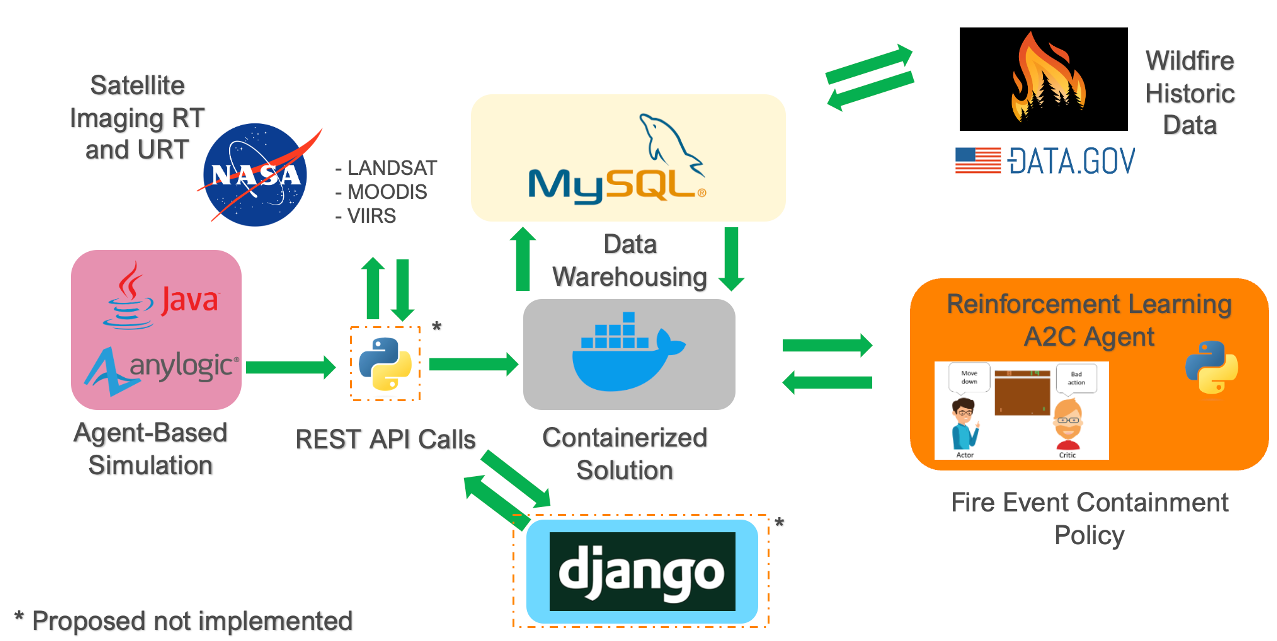
\includegraphics[height=6cm,width=12cm]{Arch.png}
  \caption{
    System Architecture: The illustration depicts the fundamental components of this digital twin. Initially, satellite imaging is employed from three sources—Landsat, MODIS, and VIIRS. Each dataset is standardized, offering a confidence level for the likelihood of a fire event at each represented heat point in the future. This data is presented in tabular format and forms the basis for the backend, comprising a Django-based API and a containerized MySQL platform. The API operates as a RESTful interface for socket communication and serves as an executor of operations within the inner backend. Real-time traffic information is sourced from TomTom live data, communicating with the OSRM routing engine to generate a realistic cost matrix for transportation in optimizing neighboring station placement. Following optimization, the results are visualized in the AnyLogic GUI. The second stage involves a reinforcement learning-based policy aiming to select the policy that minimizes the economic impact caused by a fire event. An advantage actor-critic is utilized to train independent clusters for each agent, empowering them to decide on the necessary containment actions for fire events. }\label{fig:arch}
  
\end{figure*}

\section{Problem Description}\label{Problem Description}

% \subsection{Stage 1}
% Defining the most economically efficient fire response for a particular set of fires requires determining which resources should be dispatched to contain the fire at minimum cost. This constitutes an optimization problem that lends itself to Integer Programming (IP) because fire-fighting resources are indivisible units and are dispatched accordingly.


% \subsection{Stage 2}

critical challenge is the limited effectiveness of traditional strategies in rapidly evolving and dynamic fire scenarios. Conventional approaches often struggle to adapt to the unpredictable nature of wildfires, leading to suboptimal resource allocation, delayed decision-making, and increased environmental impact
Additionally, the lack of real-time decision support systems hampers the ability of firefighting teams to respond swiftly and effectively
Develop an innovative solution that seamlessly integrates digital twins, simulation-based methodologies, and real-time deep reinforcement learning to address the shortcomings of existing wildfire management approaches. This solution aims to provide actionable insights, improve resource utilization, and minimize the environmental impact of firefighting operations, ultimately contributing to a more adaptive and proactive wildfire management paradigm

% \subsection{Simulation}


% For the simulation process we utilize four agents that represent: Heatpoints, these are entailed to generate the fire events and are created on the basis of  





\section{Methodology}\label{Methodology}

\begin{figure*}[!t]
	\normalsize % Adjust font size if necessary
	\begin{description}
	  \item[$\theta$:] Parameters of the policy function.
	  \item[$\phi$:] Parameters of the state-value function.
	  \item[$\pi(a|s;\theta)$:] Policy function representing the probability of taking action $a$ in state $s$ with parameters $\theta$.
	  \item[$R_t$:] Return at time $t$ (sum of discounted rewards over time).
	  \item[$\gamma$:] Discount factor.
	  \item[$A_t$:] Advantage function at time $t$, representing the advantage of taking action $a_t$ in state $s_t$.
	  \item[$V(s;\phi)$:] State-value function with parameters $\phi$.
	\end{description}
	
  
  
	The A2C objective function is given by:
  
  
	\begin{align}
	&L(\theta, \phi) = \sum_{t=0}^{T} \left( \log \pi(a_t|s_t;\theta) \cdot A_t + \beta \cdot \text{H}(\pi(\cdot|s_t;\theta)) \right. \left. - \alpha \cdot \frac{1}{2} (V(s_t;\phi) - R_t)^2 \right)
  \end{align}
  
  
	Where:
  
	\begin{align}
	&\text{H}(\pi(\cdot|s_t;\theta)) \text{ is the entropy regularization term,} \\
	&\beta \text{ is the entropy regularization coefficient,} \\
	&\alpha \text{ is the coefficient for the value function loss.}
	\end{align}
	\end{figure*}
  % \subsection*{Advantage Actor-Critic (A2C)}
  
  % The advantage actor-critic algorithm is a reinforcement learning technique that incorporates features of both policy gradient and value function approaches. A2C's mathematical formulation entails establishing the policy, value function, and objective function. The objective is to maximize this function with respect to the policy parameters  $\theta$ and the value function parameters  $\phi$.
  % This mehtod is represented as follows:
  
  
  % \begin{description}
  %   \item[$\theta$:] Parameters of the policy function.
  %   \item[$\phi$:] Parameters of the state-value function.
  %   \item[$\pi(a|s;\theta)$:] Policy function representing the probability of taking action $a$ in state $s$ with parameters $\theta$.
  %   \item[$R_t$:] Return at time $t$ (sum of discounted rewards over time).
  %   \item[$\gamma$:] Discount factor.
  %   \item[$A_t$:] Advantage function at time $t$, representing the advantage of taking action $a_t$ in state $s_t$.
  %   \item[$V(s;\phi)$:] State-value function with parameters $\phi$.
  % \end{description}
  % % \begin{align}
  % % &\theta \text{ : parameters of the policy function} \\
  % % &\phi \text{ : parameters of the state-value function} \\
  % % &\pi(a|s;\theta) \text{ : policy function representing the probability of taking action } a \text{ in state } s \text{ with parameters } \theta, \\
  % % &R_t \text{ : return at time } t \text{ (sum of discounted rewards over time),} \\
  % % &\gamma \text{ : discount factor,} \\
  % % &A_t \text{ : advantage function at time } t \text{, representing the advantage of taking action } a_t \text{ in state } s_t, \\
  % % &V(s;\phi) \text{ : state-value function with parameters } \phi.
  % % \end{align}
  
  % The A2C objective function is given by:\\
	
  
  % \begin{multline}
  % L(\theta, \phi) = \sum_{t=0}^{T} \left( \log \pi(a_t|s_t;\theta) \cdot A_t + \beta \cdot \text{H}(\pi(\cdot|s_t;\theta)) \right. \\
  % \left. - \alpha \cdot \frac{1}{2} (V(s_t;\phi) - R_t)^2 \right),
  % \end{multline}
  % where:
  % \begin{align}
  % &\text{H}(\pi(\cdot|s_t;\theta)) \text{ is the entropy regularization term,} \\
  % &\beta \text{ is the entropy regularization coefficient,} \\
  % &\alpha \text{ is the coefficient for the value function loss.}
  % \end{align}
  
  
  
  
  \section{Experimentation}\label{Experimentation}
  
  
  \subsection{Data Sources}
  The system's information architecture is enriched through the judicious integration of diverse datasets, notably leveraging FIRMS (Fire Information for Resource Management System). This repository provides real-time and pertinent information on active fires, affording the system a dynamic understanding of ongoing fire events. Complementing this, the incorporation of data from Open Fire Stations enhances the spatial awareness of existing fire station locations, thereby facilitating the optimization of neighboring station placements. Furthermore, the system draws insights from original sources, notably the United States Forest Service, establishing a foundation rooted in authoritative forestry data. This comprehensive amalgamation of information from FIRMS, Open Fire Stations, and original sources contributes to the system's scholarly rigor, ensuring a nuanced understanding of the multifaceted variables inherent in fire event management and response.
  The system enhances its data foundation through integration with Data.gov, a reputable source providing diverse datasets. By incorporating historical fire event registries from Data.gov, the system gains valuable insights into past incidents, enabling a nuanced analysis of patterns and trends for more informed decision-making in fire event management.
  
  \subsection{Neighboring Station}
  
  
  The determination of neighboring fire stations is derived through the following formulation, structured around a supply-demand schema. Its objective is to ascertain the optimal number of fire stations capable of responding to a fire event based on a designated index referred to as the fire\_index. This index integrates various factors obtained from independent data sources, which have been precomputed for experimental accuracy. The formulation details are provided in the subsequent lines:
  
  
  
  % \begin{figure*}[!t]
  
  % \textbf{Sets:}
  
  % \begin{description}
  %   \item[$S$:] Suppliers
  %   \item[$D_{\text{mean}}:$] Locations (mean demand)
  %   \item[$D_{\text{stddev}}:$] Standard deviations for demand
  %   \item[\texttt{combined\_param}:] Cost matrix
  % \end{description}
  
  % \textbf{Parameters:}
  % \begin{description}
  %   \item[\texttt{num\_suppliers}:] Number of suppliers
  %   \item[\texttt{num\_demand\_points}:] Number of demand points
  % \end{description}
  
  % \textbf{Constraints:}
  % \begin{description}
  %   \item[Supply Constraints:] $\sum_{j} x[i, j] \leq S[i]$ for each supplier $i$
  %   \item[Demand Constraints:] $\sum_{i} x[i, j] = D[j]$ for each demand point $j$
  % \end{description}
  
  % \textbf{Objective Function:}
  % \begin{equation}
  %     \text{Minimize } \sum_{i,j} \text{combined\_param}[i][j] \times x[i, j]
  % \end{equation}
  % \end{figure*}
  
  
  
  
  \subsection{Fire Containment}\label{Fire Containment}
  
  \begin{figure}
	\centering
	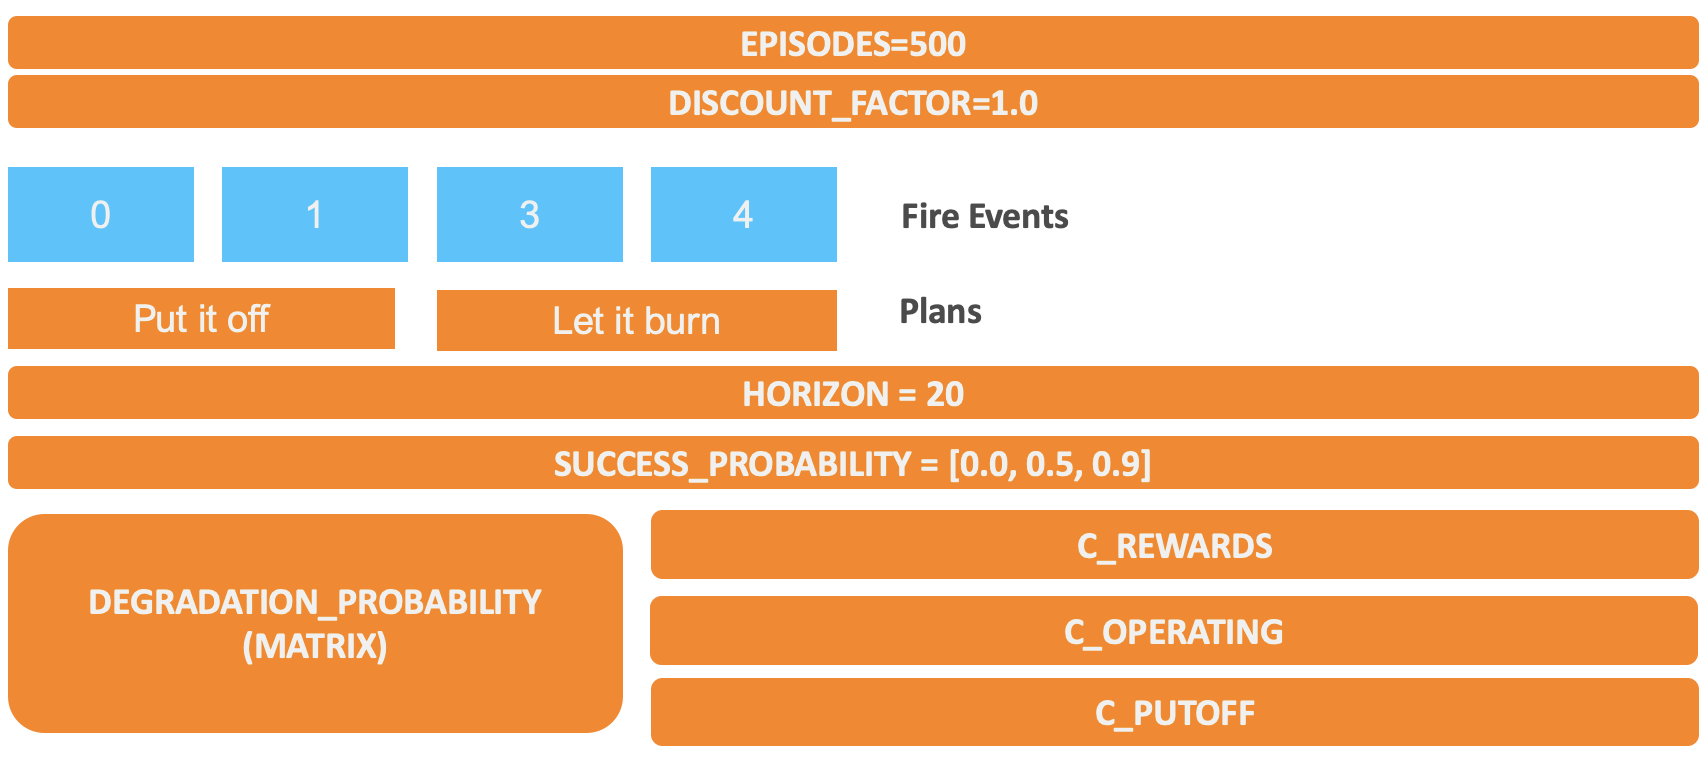
\includegraphics[height=5cm,width=8cm]{parameters.png}
	\caption{Deep Reinformcement Leanring Parameters: The experimental parameters are configured as follows: \texttt{EPISODES=50000} dictates the number of agent simulations for policy improvement; \texttt{DISCOUNT\_FACTOR=1.0} emphasizes the full consideration of future rewards; \texttt{seed\_value = 42} ensures reproducibility through a set seed for the random number generator. \texttt{num\_states = Max\_FirePoints} signifies the count of environmental states, often representing diverse fire scenarios or locations. \texttt{num\_plans = 2} denotes the available action choices for the firefighter, likely relating to deciding whether to address a fire. \texttt{T = 20} defines the time horizon, indicating the number of time steps before updating policies or the simulation duration. \texttt{success\_pr = [0.0, 0.5, 0.9]} characterizes the success probability of extinguishing a fire, with values indicating varying success levels. The \texttt{degrade\_pr} matrix portrays degradation probabilities for each state, reflecting the likelihood of environmental deterioration. \texttt{C\_reward = 10} denotes the reward for fire prevention per time step, incentivizing a safe environment. \texttt{C\_Operating} encapsulates operating costs, suggesting state-dependent variations. \texttt{C\_Putoff} captures put off costs, contingent on the chosen action, likely reflecting the expenses associated with fire suppression strategies. }
  \end{figure}
  
  
  
  \begin{figure}
	\centering
	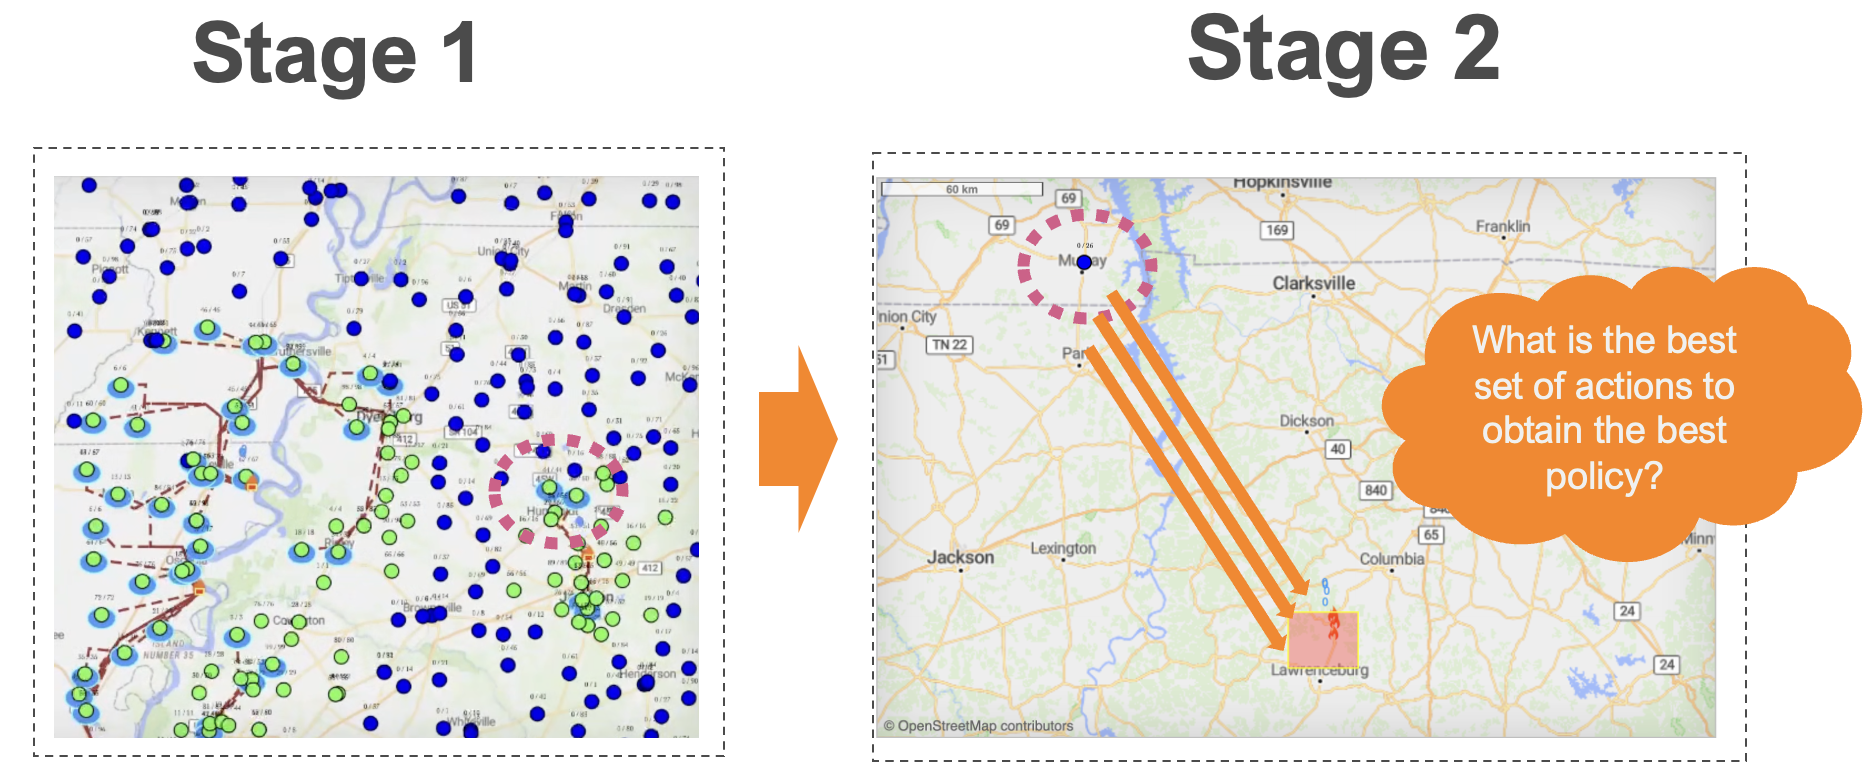
\includegraphics[height=4cm,width=9.5cm]{stages.png}
	\caption{Stages Transfering: We illustrate the process of transitioning from the initial stage to the subsequent deep reinforcement learning (DRL) model in a two-stage framework. Initially, our Neighboring approach strategically allocates the requisite number of fire stations to address the prevailing number of fire events in a given area. The fire stations surrounding each fire event are then clustered, constituting Stage two. In this stage, the individual fire stations and associated resources are treated as a unified entity. The DRL approach subsequently formulates a policy, determining the optimal actions for each fire event—whether to contain, extinguish, or withhold resource allocation—at discrete time intervals, starting at $t=0$. Visualized through three arrows, these actions represent the various states the agent (comprising a cluster of fire stations and resources) can assume during the second stage. Our temporal horizon spans 20 time steps, with each step equivalent to an hour in Anylogic units, providing a comprehensive representation of the evolving dynamics.}\end{figure}
  
  
  \begin{figure}
  \centering
  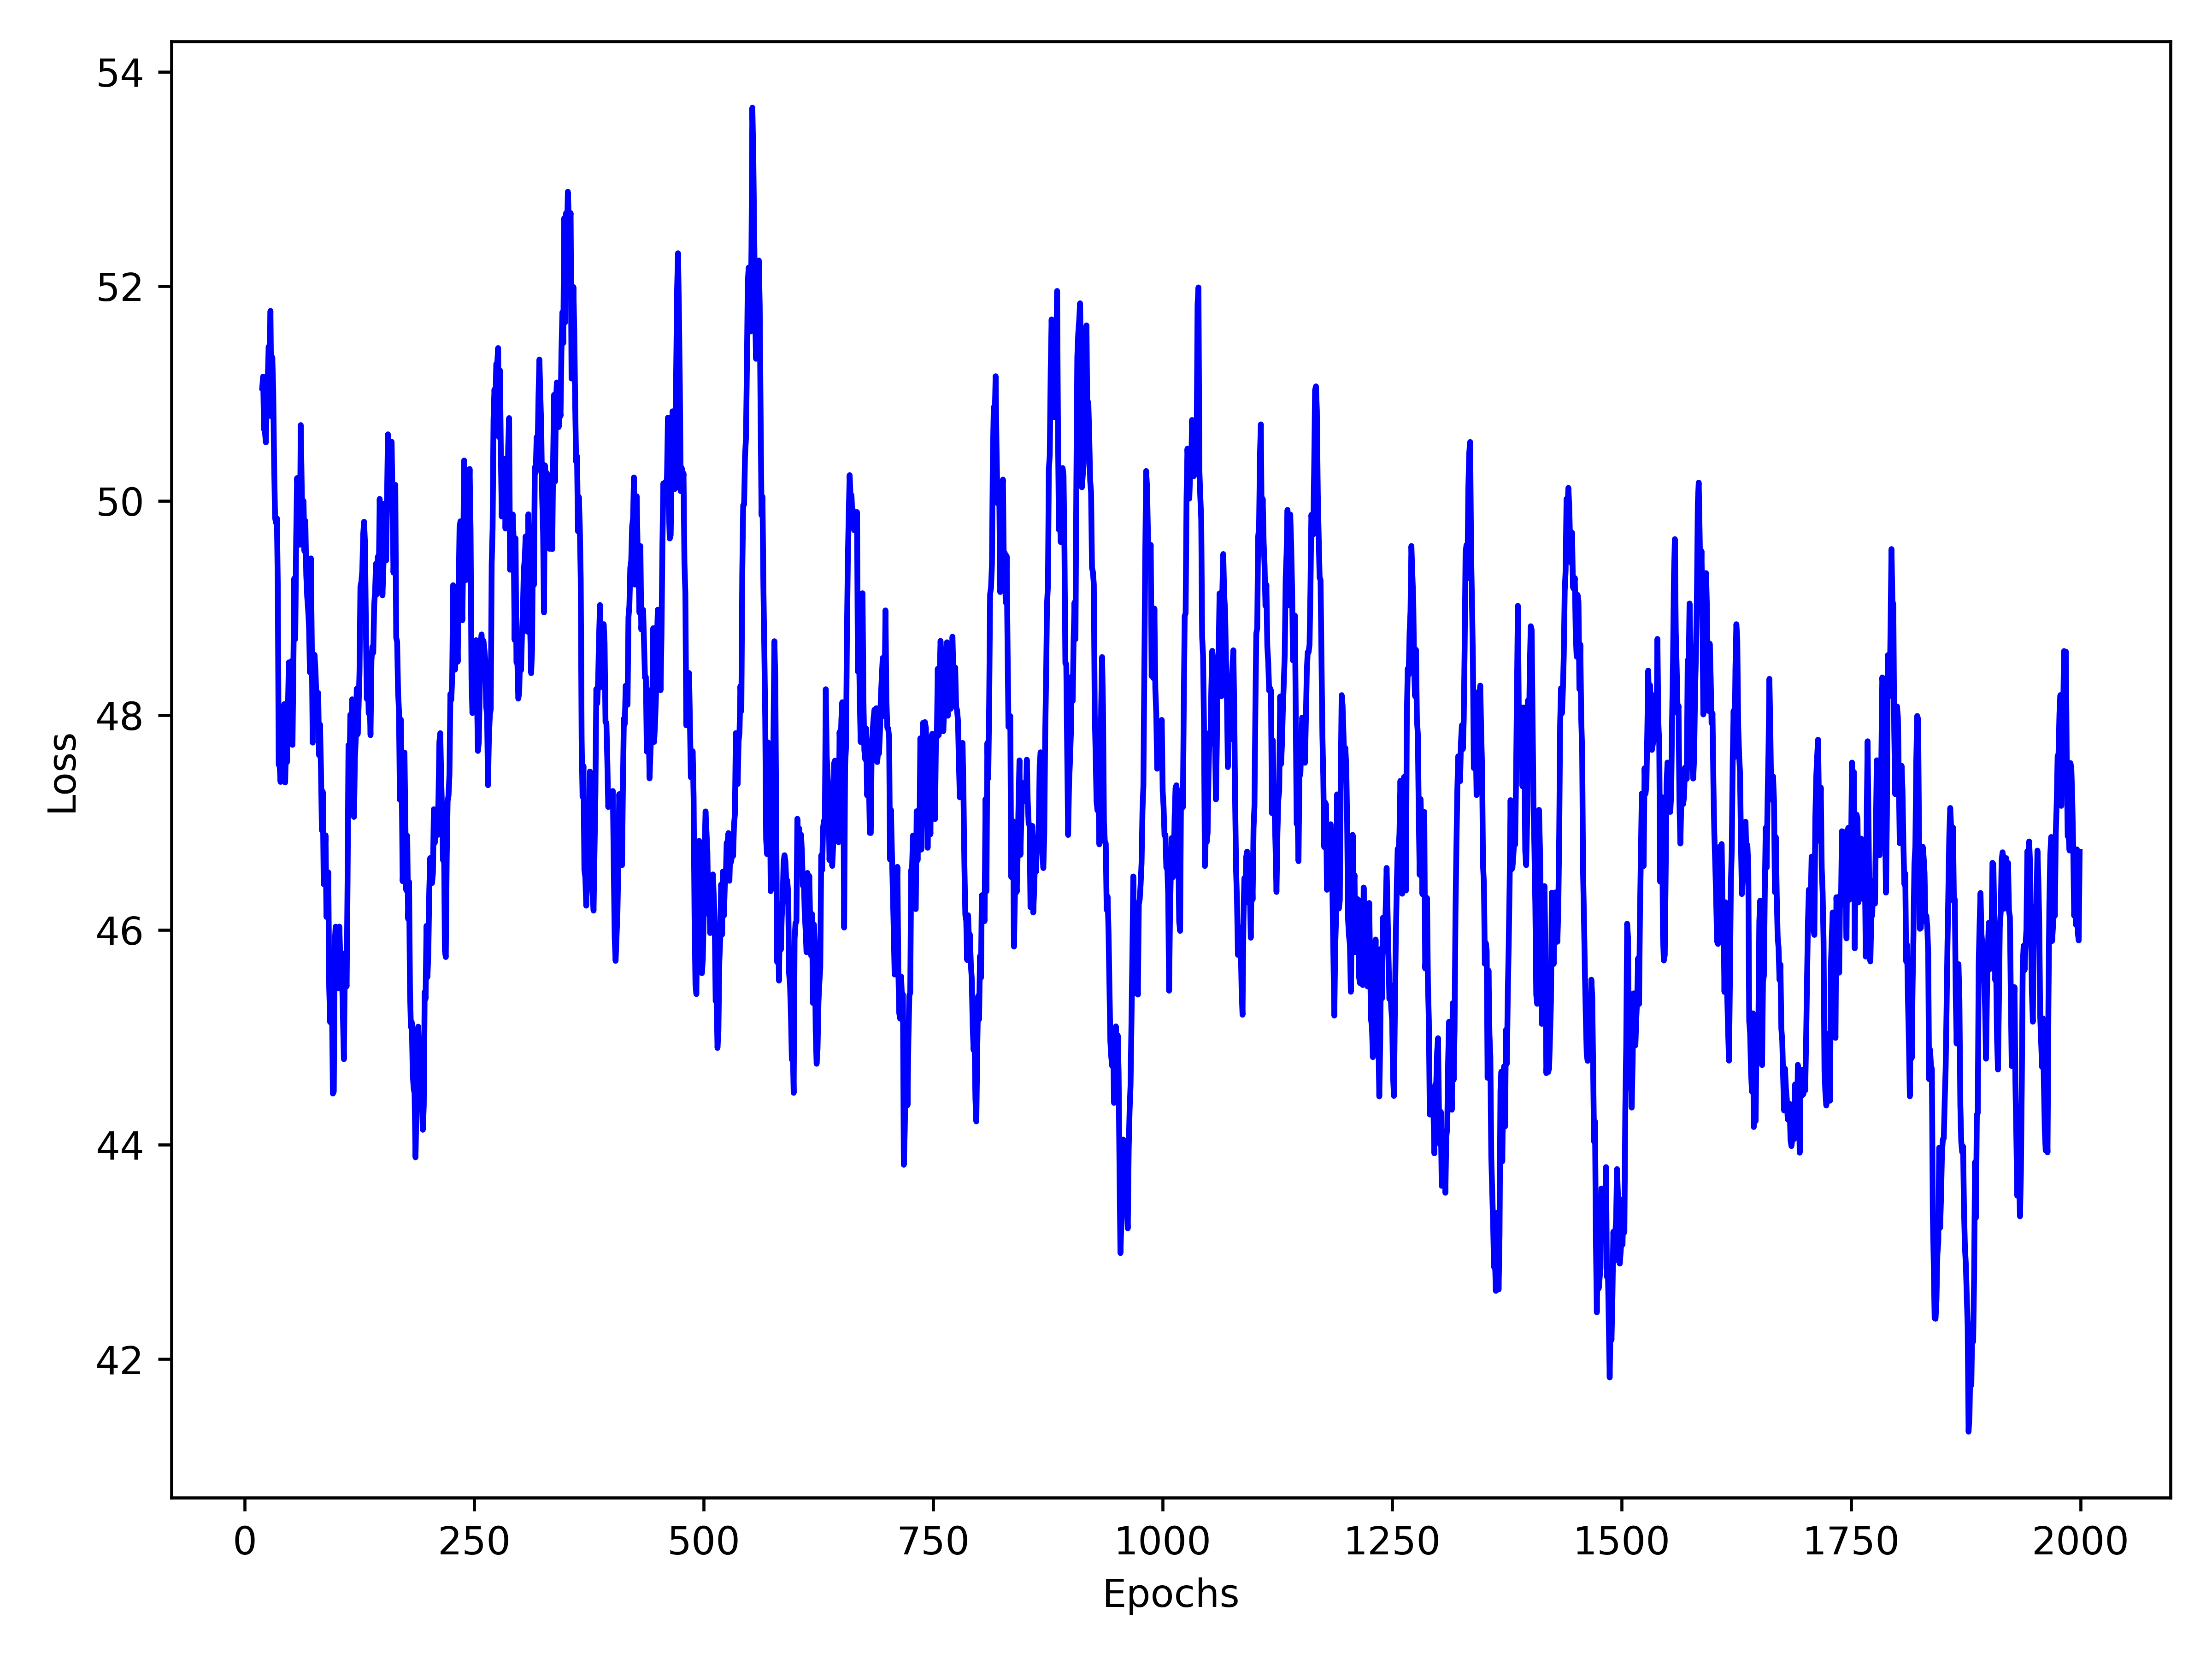
\includegraphics[height=4cm,width=8cm]{manager_actor_loss.png}
  \caption{Actor Loss: It indicates the cost of training the policy network. The actor loss leads policy modification to raise the likelihood of actions leading to better returns and decrease the likelihood of actions leading to lower returns. It is a component of the overall loss function, which combines actor and critic losses with the goal of maximizing the predicted cumulative reward by changing both the policy and value functions. }\end{figure}
  
	
  
  \begin{figure}
  \centering
  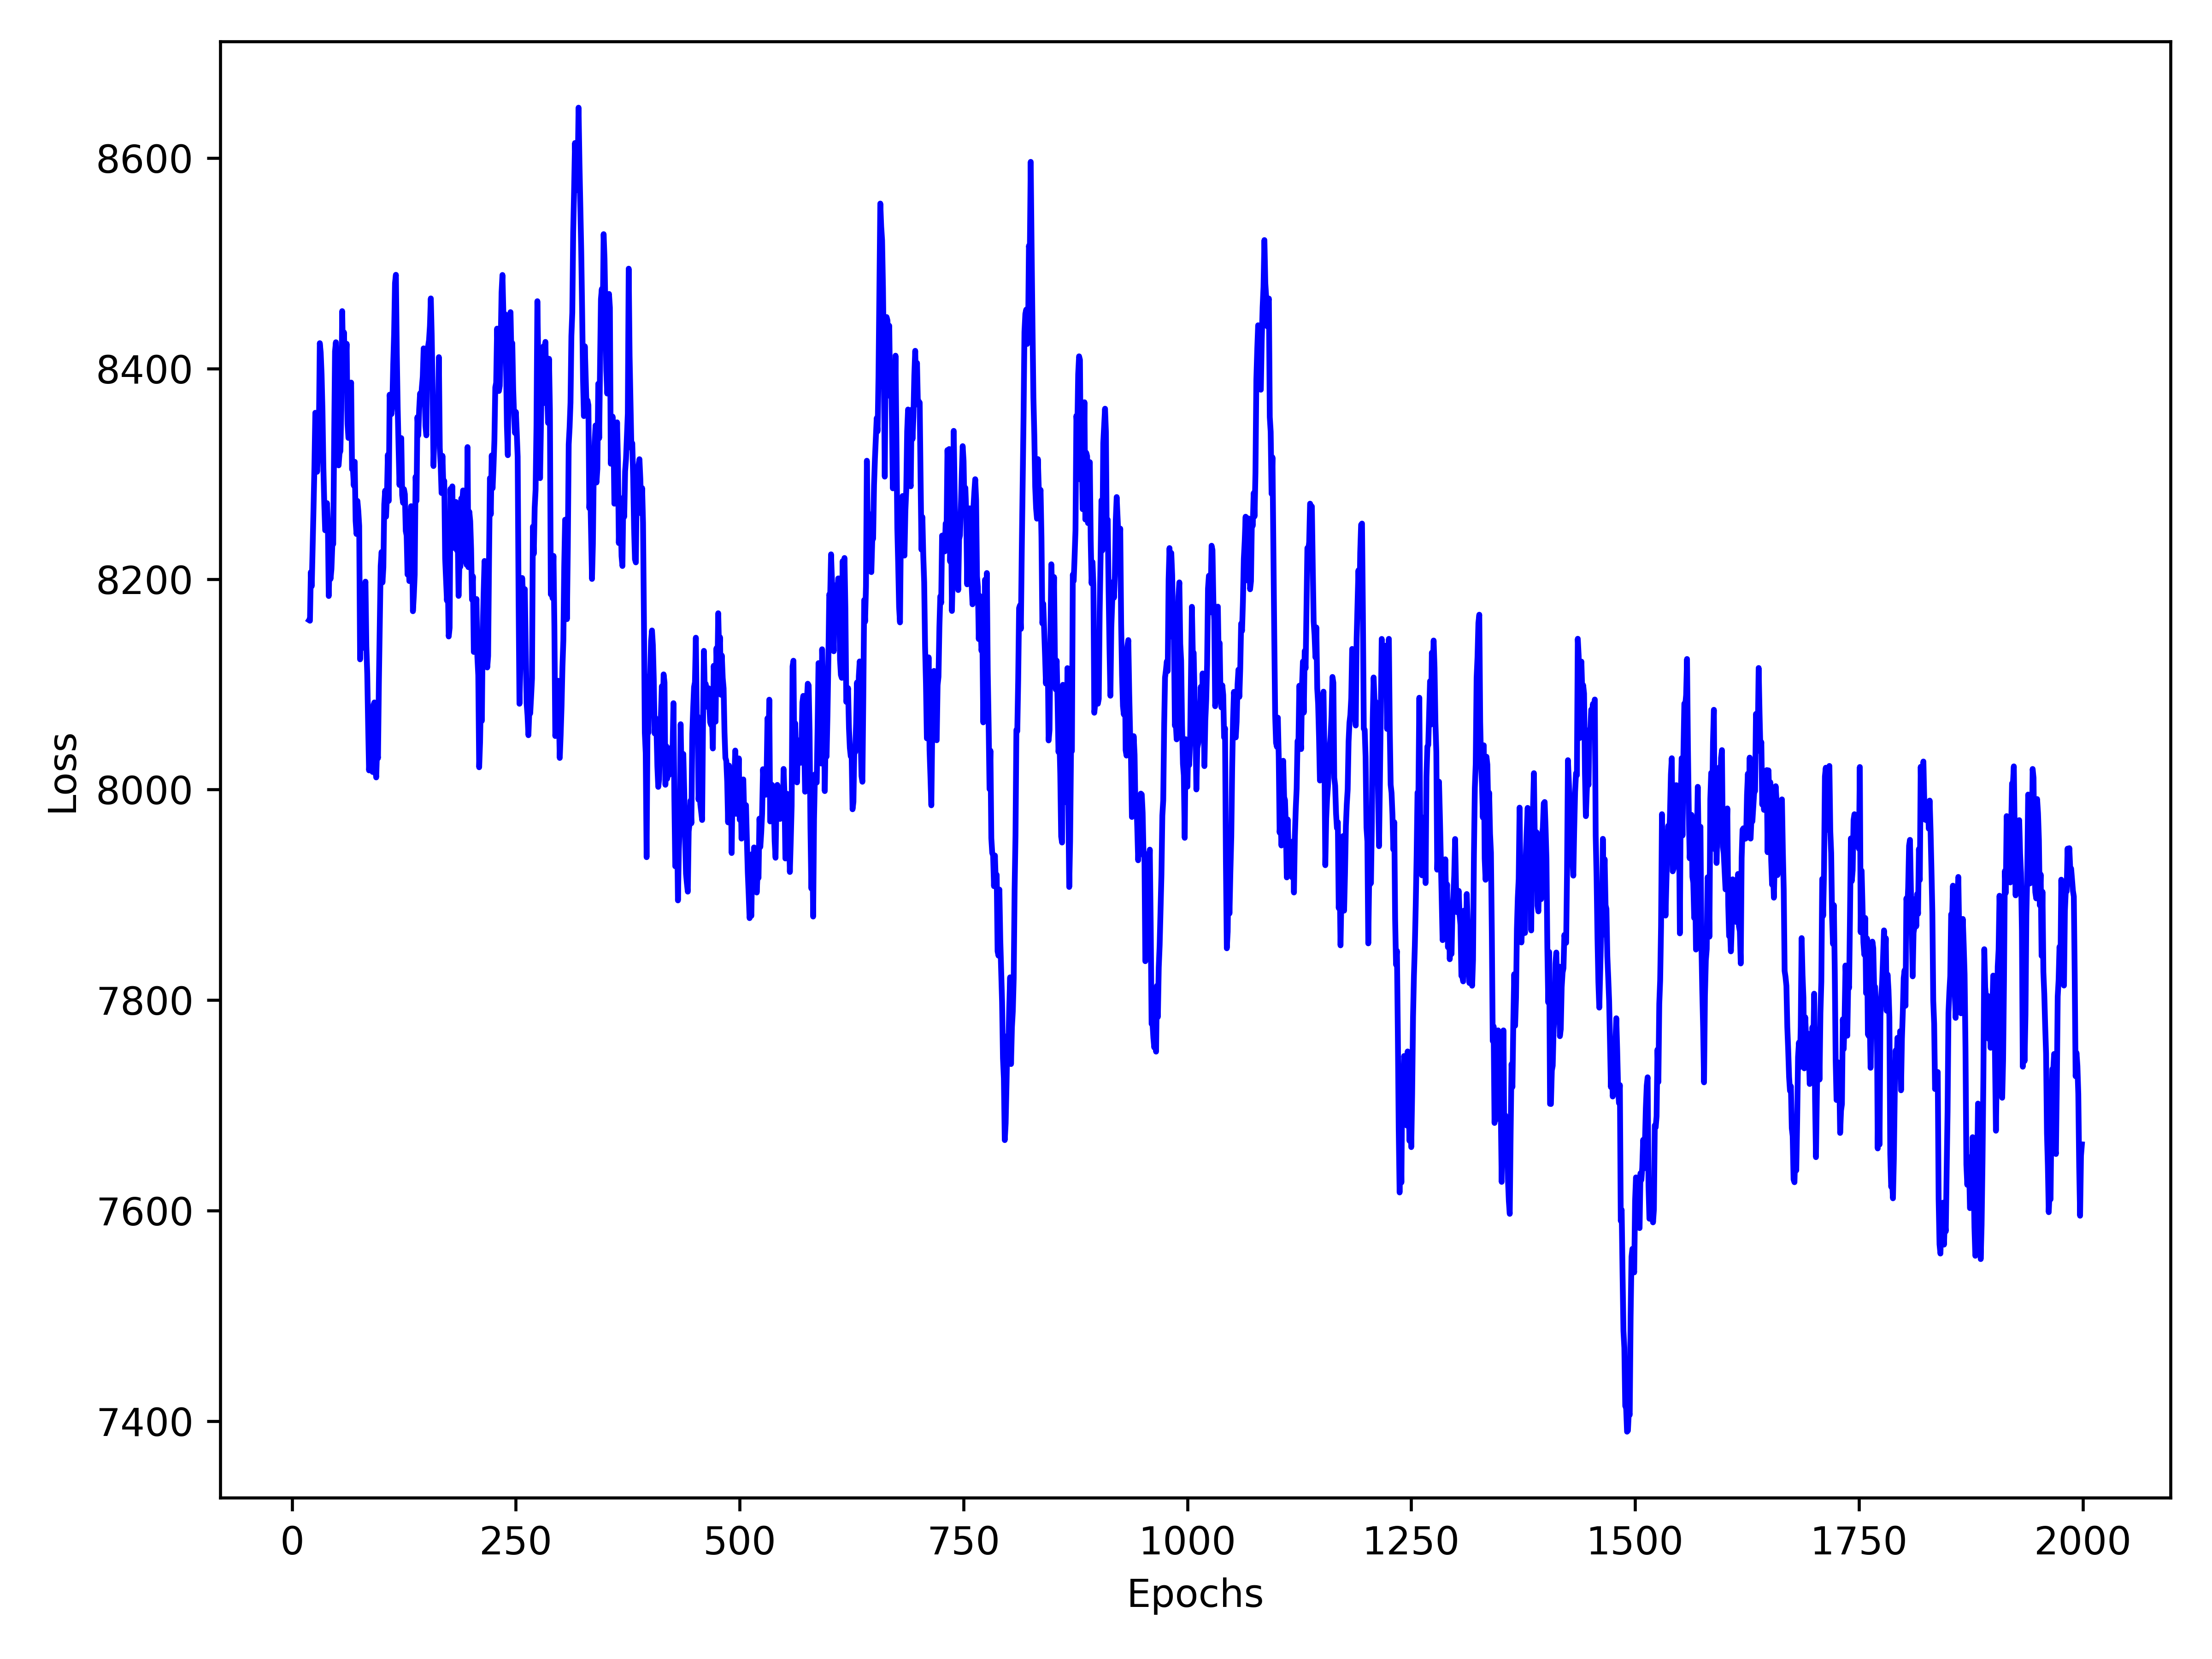
\includegraphics[height=4cm,width=8cm]{manager_critic_loss.png}
  \caption{Critic Loss: In Advantage Actor-Critic (A2C), the critic loss indicates the difference between the projected state value and the actual return seen during reinforcement learning training. The critic is in charge of estimating the state-value function, which calculates the predicted cumulative reward from a particular condition in A2C. The critic loss, which is frequently expressed as the mean squared error between the anticipated state value and the actual return, is a measure of how well the critic's predictions match the genuine rewards received in the environment.}\end{figure}
	  
	  
		\begin{figure}
		  \centering
		  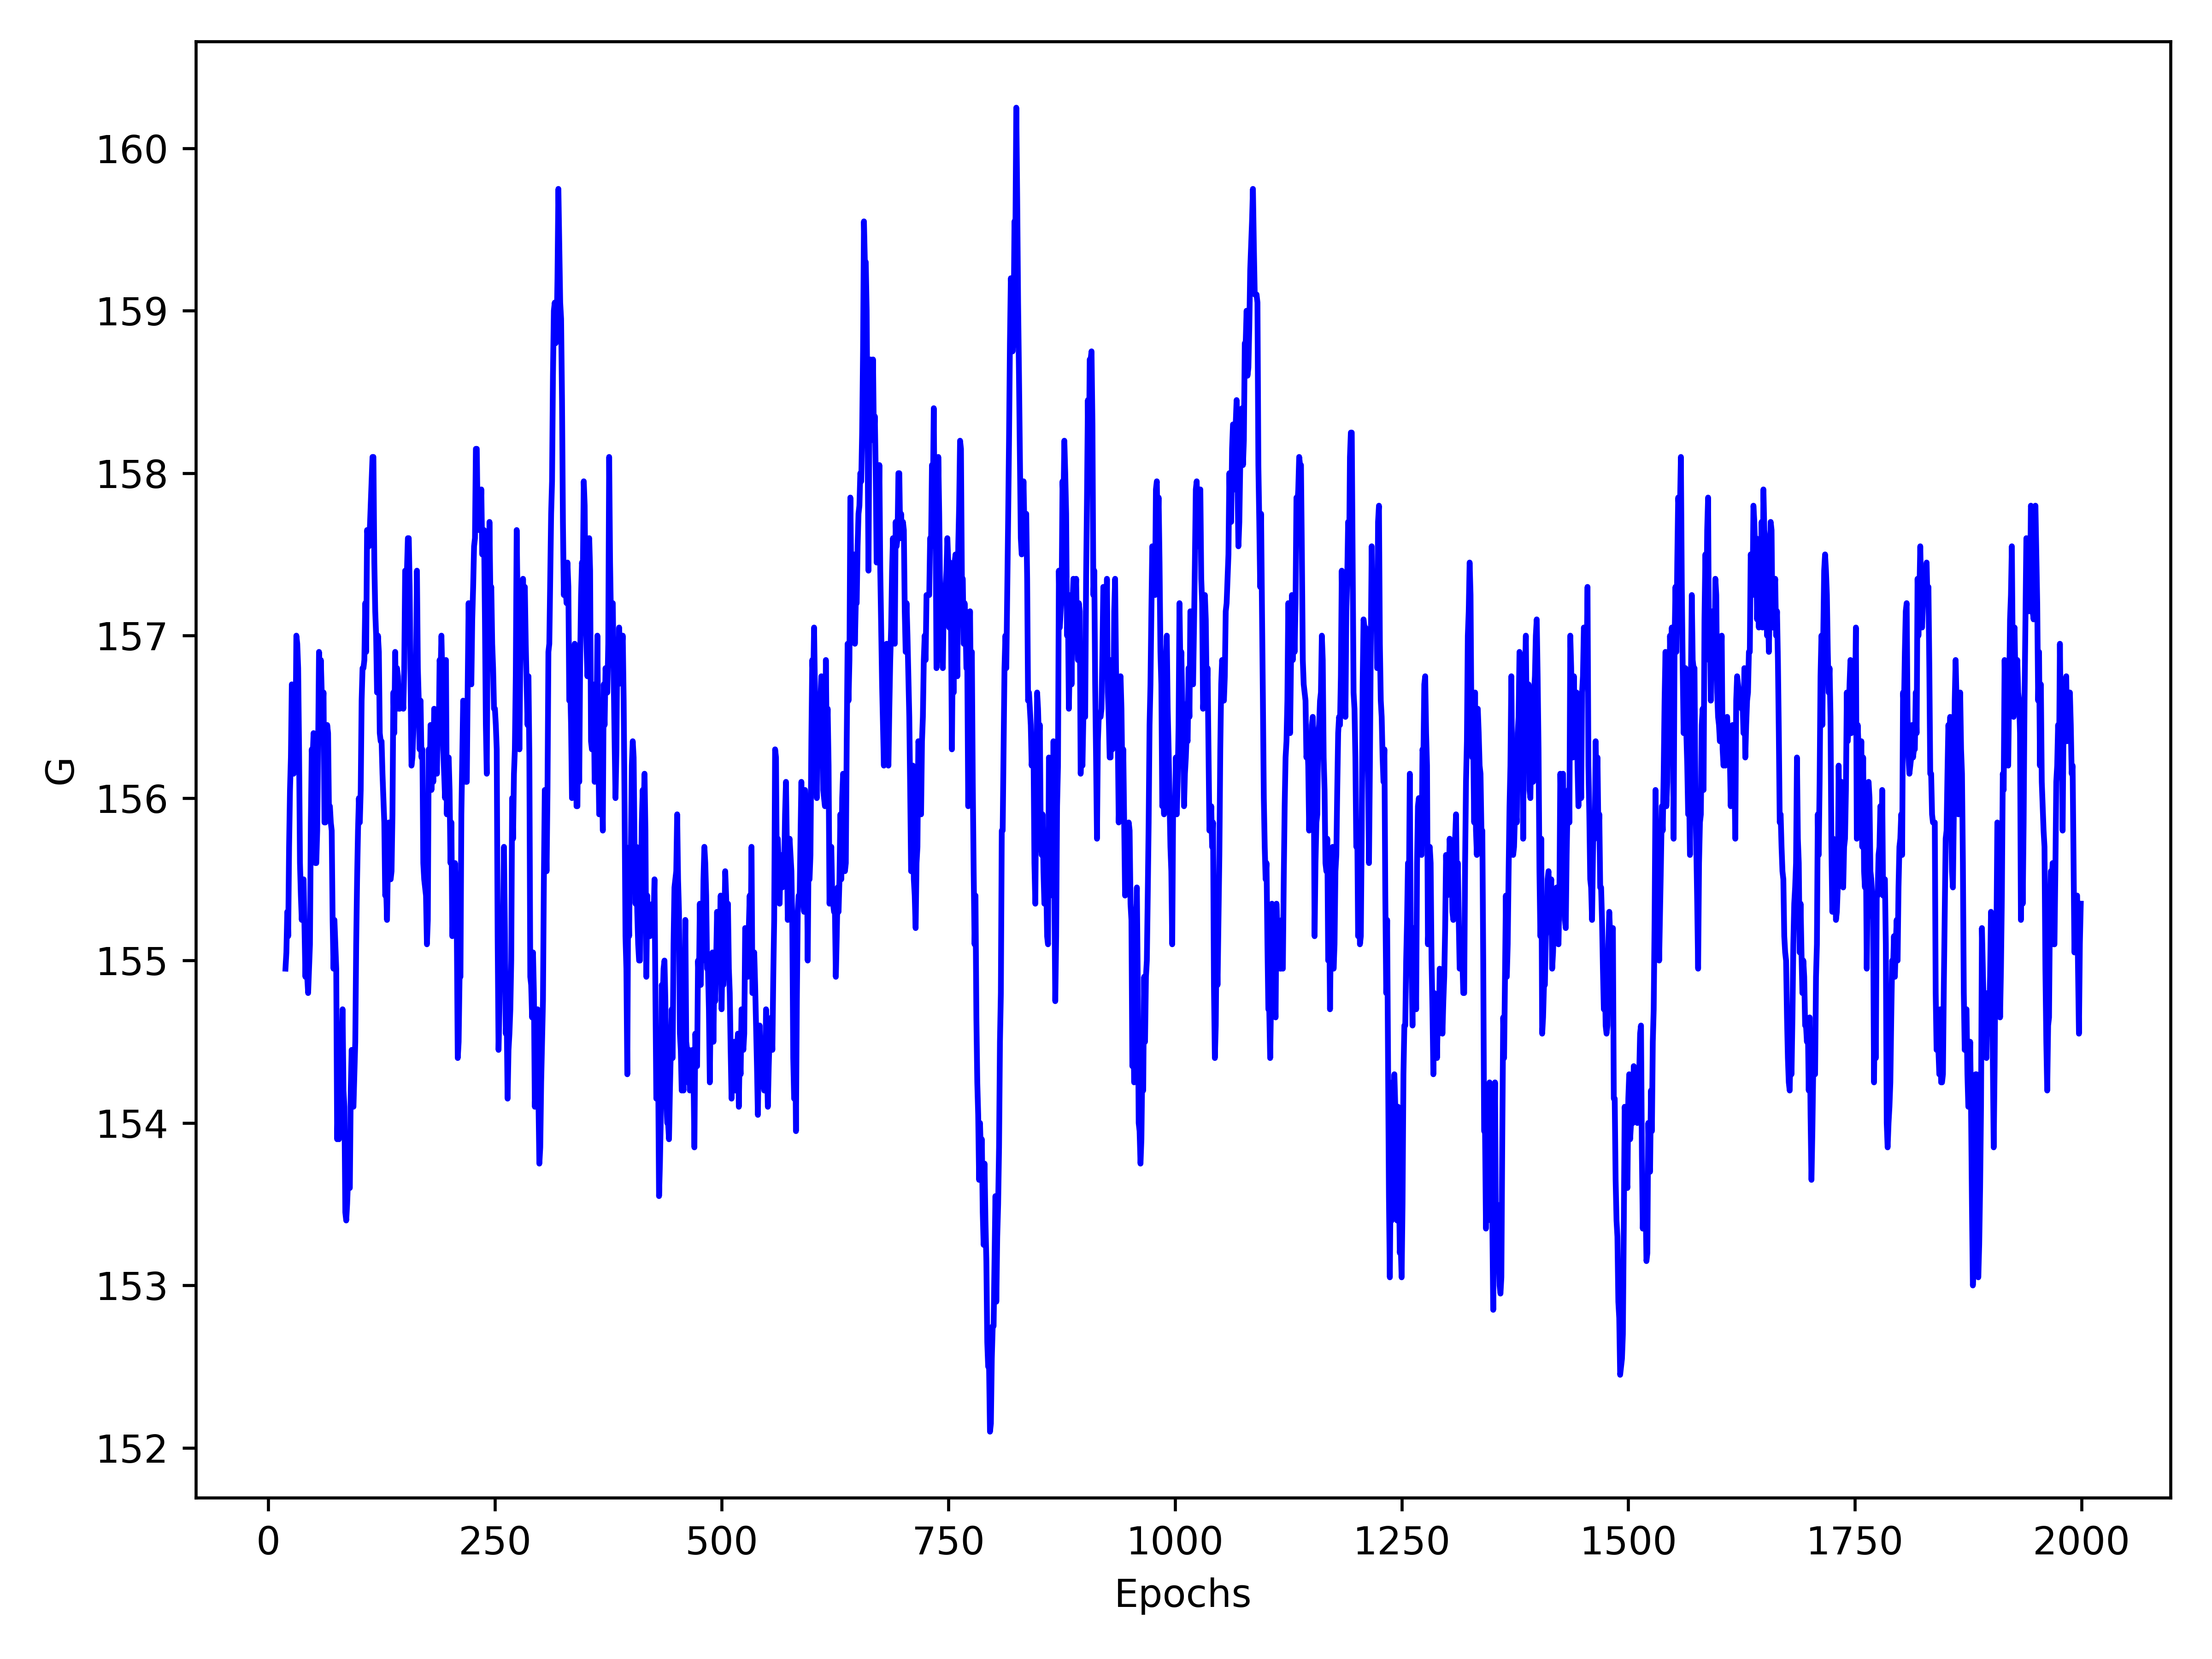
\includegraphics[height=4cm,width=8cm]{manager_G.png}
		  \caption{This section elucidates the profound impact of actions on the overarching policy return. A well-converged model is anticipated to showcase a discernibly smoother pattern, contrasting with the inherent noise observed during earlier stages. The graphical representation serves to illustrate the pivotal role actions play in shaping the cumulative return of the policy, offering insights into the stability and effectiveness achieved through convergence.}\end{figure}
		
		
		  \begin{figure}
			\centering
			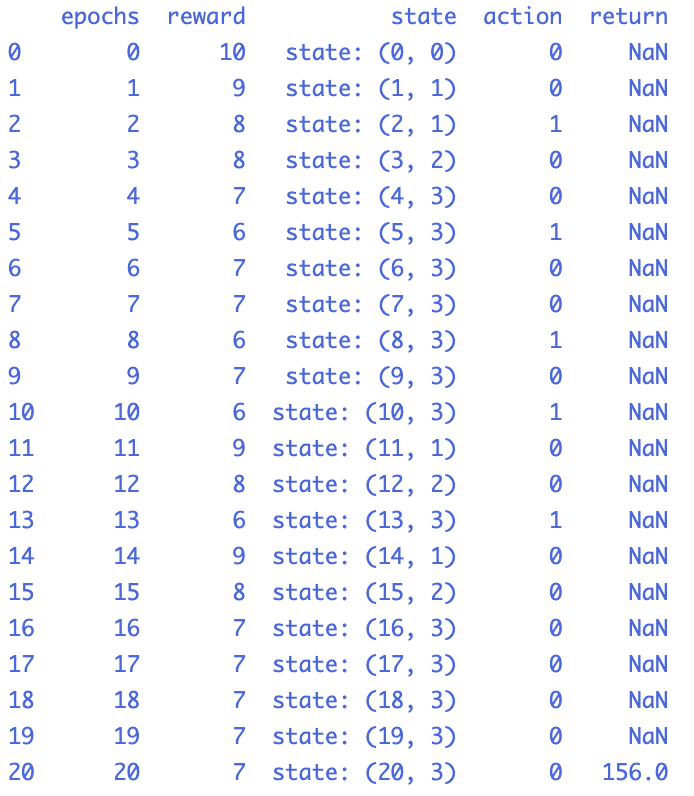
\includegraphics[height=5cm,width=5cm]{4_2000.png}
			\caption{Action Schema: This comprehensive depiction provides a detailed examination of state rewards, actions, and individual states. To navigate the intricacies of the data, it is advisable to implement a state-action filter to prevent unnecessary traversal through events where fires have already been extinguished. Notably, an observable pattern emerges, highlighting the effective control measures applied to fire event 3, also denoted as state 3, which demonstrate a successful containment strategy deployed multiple times.}\end{figure}
		  
		  
		
  
			\begin{table}
			  \centering
			  \caption{This table represents the results of various test events conducted to assess system performance. Five distinct tests were executed, systematically increasing the number of fire events to evaluate their impact on the overall system return. Notably, our analysis focused on a carefully selected cluster of data points.
			  For this specific cluster, it became evident that exceeding eight fire events would likely surpass the capacity of the fire points cluster, inevitably leading to repercussions on the population. It is crucial to emphasize that the policies implemented during these tests are still in the developmental phase. Ongoing efforts are directed towards further refinement and completion in the subsequent stages of this research.
			  These findings underscore the need for cautious consideration and ongoing optimization as we progress in the development of robust policies for managing fire events.
			  }
			  
			  
			  \begin{tabular}{|c|c|c|}
				\hline
				\textbf{Test} & \textbf{Fire Events} & \textbf{Return} \\
				\hline
				1 & 4 & 156 \\
				2 & 8 & 97 \\
				3 & 80 & -961 \\
				4 & 100 & -1224 \\
				5 & 800 & -11465 \\
				\hline
				\end{tabular}
			\end{table}
  
  


\section{Conclusion \& Further Directions}

The presented approach outlines a comprehensive digital twin framework for wildfire management that leverages various innovative technologies. The integration of parameterized experiments facilitates the strategic allocation of firefighting entities to neighboring areas, guided by a novel fire station index. The utilization of deep reinforcement learning is a key highlight, as it determines optimal policies for clustered fire stations, aiming to minimize the impact of wildfires on the population. This not only enhances the efficiency of firefighting scenarios but also demonstrates a forward-looking approach to addressing dynamic and complex challenges.

The incorporation of real-time data from satellite imaging and a routing engine further enhances decision-making capabilities, allowing for a more accurate and timely response to evolving wildfire situations. By integrating these technologies, the framework creates a holistic and adaptive response system. The emphasis on deep reinforcement learning throughout the system signifies a commitment to effective wildfire management through continuous learning and optimization. This approach represents a significant step towards leveraging cutting-edge technologies for more efficient, data-driven, and adaptive wildfire management strategies.



% This paper provides instructions for the preparation of papers for the Society for Modeling \& Simulation International (SCS) using \LaTeX. 
% %There is a companion paper that provides instructions for the preparation of papers with Microsoft Word.
% The easiest way to write a paper using \LaTeX\ that complies with the requirements is to edit the source file, \texttt{scs23paper.tex} for this document. Please do not use an older version, as some specifications may have changed. An author kit is available via the conference website, including this \LaTeX\ document. 
% %and its Microsoft Word companion.
% %This document was typeset using \texttt{pdflatex}.

% \section{General Guidelines}

% \subsection{Language}

% The paper should be prepared using U.S. English to ensure consistency across the proceedings. Please carefully check the spelling of words before you submit your paper. There are spell checkers for \LaTeX\ as well.
% Some examples of software that supports spell-checking are TexnicCenter, TexMaker, and TexClipse.

% \subsection{Objectivity}
% The paper's content should be objective and without any appearance of commercialism.  Comparisons of commercial software should be avoided unless they are central to the topic.  If a comparison of commercial software is included, it should be based on objective analysis that provides for criteria, a description of ranking methodology on each criterion, and the rankings themselves to arrive at the conclusion.
% If an approach other than a detailed objective analysis is used to select the simulation software used for the study being reported, such as the availability of the software, or the familiarity of the analyst with the software, it should be clearly identified. To ensure suitability for an international audience, please pay attention to the following:

% \begin{itemize}
% \item{Write in a straightforward style.}
% \item{Try to avoid long or complex sentence structures.}
% \item{Briefly define or explain all technical terms that may be unfamiliar to readers.}
% \item{Explain all acronyms the first time they are used in your text – e.g., “Digital Signal Processing (DSP)”.}
% \item{Explain local references (e.g., not everyone knows all city names in a particular country).}
% \item{Explain “insider” comments. Ensure that your whole audience understands any reference whose meaning you do not describe (e.g., do not assume that everyone has used a Macintosh or a particular application).}
% \item{Explain colloquial language and puns. Understanding phrases like “red herring” may require a local knowledge of English. Humor and irony are difficult to translate.}
% \item{Use unambiguous forms for culturally localized concepts, such as times, dates, currencies and numbers (e.g., “1-5- 97” or “5/1/97” may mean 5 January or 1 May, and “12/10/11” can be even more confusing, and “seven o’clock” may mean 7:00 am or 7:00 pm).  For currencies, indicate English equivalences – e.g., “Participants were paid 10,000 lire, or roughly \$5.”}
% \item{Be careful with the use of gender-specific pronouns (he, she) and other gendered words (chairman, manpower, man-months). Use inclusive language that is gender-neutral (e.g., she or he, they, s/he, chair, staff, staff-hours, person-years).}
% \item{If possible, use the full (extended) alphabetic character set for names of persons, institutions, and places (e.g., {Gr\o nb\ae k}, Lafreni\'ere, S\'anchez, Universit\"at, {Wei\ss enbach}, Z\"ullighoven, {\AA rhus}, etc.).}
% \end{itemize}

% \subsection{Paper Submission}

% Please, refer to the author's guidelines document in the author's kit.

% \subsection{Length Constraints}

% \subsubsection{The Abstract and Keywords}
% \textcolor{red}{The abstract should be at most 150 words.} Since abstracts of all papers accepted for publication in the proceedings will also appear in the final program, the length limit of 150 words will be strictly enforced for each abstract. The abstract should consist of a single paragraph, and it should not contain references or mathematical symbols. 

% The list of keywords should have no more than five keywords that will identify your paper in indices and databases (required). Do not use the words “computer”, “simulation”, “model”, or “modeling”, since these are all assumed.

% \subsubsection{Length of the Paper}
% The page size in the proceedings must be 8.5 inches by 11 inches (21.6 cm by 27.9 cm). The overall length of the paper should be at least 5 proceedings pages. \textcolor{red}{Papers should be at most 12 pages}.

% \subsubsection{Font Specification and Spacing}
% The paper should be set in Times New Roman font using an 11-point font size and it should be single-spaced. Do not use other fonts; the use of other fonts means the proceedings editors will need to send the paper back to you to change the font.

% These settings are automatically applied by the class file used for this document, thus you are asked not to change these settings in your paper. If you want to use bold Greek symbols you should use the \texttt{bm} package.

% \subsubsection{Margins}
% \label{sec:margins}

% The width of the text area is 6.5 inches (16.0 cm). The left and right margins should be 1 inch (2.54 cm) on each page. The top margin shall be 0.89 inches (2,24 cm) including the header, and the bottom of the pages shall be 0.67 inches (1.7 cm). These settings are automatically applied by the class file used for this document, thus you are asked not to change these settings in your paper.

% \subsubsection{Justification}

% Headings of sections, subsections, and subsubsections should be left justified. One-line captions for figures or tables should be centered. A multiline caption for a figure or table should be fully justified. All other text should be fully justified across the page (that is, the text should line up on the right-hand and left-hand sides of the page). These settings are automatically applied by the class file used for this document.

% \subsection{Headings of Sections, Subsections, and Subsubsections}

% Section, subsection, and subsubsection headings should appear flush left, set in the bold font style, and numbered as shown in this document. The headings for the Abstract, Acknowledgments, References, and Author Biographies sections are not numbered. These settings are automatically applied by the class file used for this document.

% To suppress the section numbers, use the \verb+\section*{}+ command.

% Section headings should be set in \textbf{\uppercase{full capitals like this phrase}}, while subsection and subsubsection headings should be \textbf{Capitalized
% in Headline Style like This Phrase}. These settings are automatically applied by the class file used for this document.

% \subsubsection{Paragraphs}
% The paragraphs should not be indented. The normal style will add a space between paragraphs, do not insert additional space between paragraphs.

% \subsubsection{Footnotes}
% \textbf{Do not use footnotes}; instead incorporate such material into the text directly or parenthetically.

% \subsubsection{Page Numbers}
% \textbf{Do not include page numbers.} Page numbers are generated by the proceedings editors once all accepted papers are ordered for the final proceedings.


% \section{Formatting the First Page}

% \subsection{Running Heads}
% The running head (provided in the template) in the lower left-hand corner of the first page (\textit{which should read the proceedings name, editors' name, conference name, location, and the name of the Society}) is left-justified and set in the 9-point italic font style. %You do not have to change the content of the first page copyright notice; the first page header and footer are automatically provided by the class file.
% You will need to \textbf{uncomment the appropriate version of the track or symposium name} at the beginning of \texttt{scs23paper.tex}, depending on where you are going to submit your paper.

% Running heads on the second and subsequent pages should contain the last names of the authors, centered and set in the 10-point italic font style. For example, running heads for papers with varying numbers of authors would appear like \emph{Yilmaz} (single author), or \emph{Yilmaz and Chan} (two authors), or \emph{Yilmaz, Chan, and Moon} (three authors), or \emph{Yilmaz, Chan, Moon, and Roeder} (four authors). These are created by using the following macro:

% \noindent \begin{verbatim}
% \SCSpagesetup{LastName1, LastName2, and LastNameLastAuthor}
% \end{verbatim}

% located just after the \verb+\begin{document}+ of this \texttt{.tex} file.

% Please use this macro to set up the running heads, as it sets further parameters important for the correct layout of the document. List all authors; do not use \textit{et al.} The author names are listed in the same order as they appear on the title page. This will be the same order when providing the author's biographies at the end of the paper.


% \subsection{Title and Authors}

% Center the title of the paper on the page and set it in bold 12pt \textbf{\uppercase{full capitals}}. The top edge of the title should begin at least 1.25 inches from the top of the page. The correct placement is automatically done by the class file as well. Just use the \verb+\title+ and \verb+\maketitle+ commands as it is done in the source of this document. Multiline titles should have about the same amount of text on each line. There should be 1 blank line between the title and the authors’ names (will be inserted by the class file if the \verb+\author+, \verb+\title+, and \verb+\maketitle+ commands are used).

% % Each author’s name should be centered on a new line, with the author’s first name first and no job title or honorific. Insert 1 blank line between the author’s name and address. The organization or institution that the author is affiliated with should be typed first. Next type the complete street address, without abbreviations, followed by the city, standard two-letter state or province abbreviation, and country. The address should be centered. For papers with multiple authors, the authors should be listed in order of decreasing contribution, with authors from the same institution listed jointly if possible.
% % You should use the \verb+\author+ command to enter author names, separated using the command \verb+\and+. See the \texttt{.tex} source file for this document.
% % Authors with multiple affiliations shall pick the main affiliation for the title page and mention other affiliations in their biography.

% You should use the \verb+\author+ command to enter author names. See the \texttt{.tex} source file for this document. The author’s first name should be listed first and with no job title or honorific. Use the \verb+\authorrefmark+ command with a number parameter to indicate the affiliation of each author. For multiple affiliations, use a space between these \verb+\authorrefmark+ commands. For papers with multiple authors, the authors should be listed in order of decreasing contribution.



% \section{Formatting Subsequent Pages}
% Please refer to \autoref{sec:margins} for the correct margins.

% \subsection{Mathematical Expressions in Text and in Displays}
% Display only the most important equations, and number only the displayed equations that are explicitly referenced in the text. To conserve space, simple mathematical expressions such as \mbox{$\bar Y = n^{-1} \sum_{i=1}^n Y_i$} may be incorporated into the text. Mathematical expressions that are more complicated or that must be referenced later should be displayed, as in

% \begin{equation}
% s^2 = \frac 1 {n-1} \sum_{i=1}^n (Y_i - \bar Y)^2\;. \nonumber
% \end{equation}

% If a display is referenced in the text, then enclose the equation number in parentheses and place it flush with the right-hand margin of the column. For example, the quadratic equation has the general form

% \begin{equation} \label{eq:quadratic}
% ax^2 + bx + c = 0, \mbox{ where } a \ne 0\;.
% \end{equation}

% In the text, each reference to an equation number should also be enclosed in parentheses. For example, the solution to \eqref{eq:quadratic} is given in \eqref{eq:quadratic sol} in \autoref{app:quadratic}.

% If the equation is at the end of a sentence, then you should end the equation with a period. If the sentence in question continues beyond the equation, then you should end the equation with the appropriate punctuation~-~that is, a comma, semicolon, or no punctuation mark.


% \subsection{Displayed Lists}
% A displayed list is a list that is set off from the text, as opposed to a run-in list that is incorporated into the text. The bulleted list given below provides more information about the format of a displayed list. 
% \begin{itemize}
% 	\item Use standard bullets instead of checks, arrows, etc.\ for bulleted lists.
% 	\item For numbered lists, the labels should not be Arabic numerals enclosed in parentheses because such labels cannot be distinguished from equation numbers.
% \end{itemize}

% The paragraph after the list is not indented.
% \begin{enumerate}
% 	\item Use standard numbering instead of special characters for numbered lists.
% 	\item For numbered lists, the labels should not be Arabic numbers enclosed in parentheses because such labels cannot be distinguished from equation numbers.
% 	\item You may need to restart the numbering on numbered lists.
% \end{enumerate}


% \subsection{Definitions and Theorems}
% Definitions, theorems, propositions, etc. should be formatted like a normal paragraph with a boldface heading as shown in the examples below. Number these items separately and sequentially. You may choose to separate number theorems, propositions, corollaries, etc., as opposed to the example below where corollaries and theorems are numbered together. Search the source of this document to see how these environments were defined. The key command is \verb+\newtheorem+. Use a period after the definition, theorem, corollary, or proposition number.

% \begin{definition}
% In colloquial New Zealand English, the term \emph{dopey mongrel} is used to refer to someone who has exhibited less than stellar intelligence.
% \end{definition}

% \begin{theorem}
% If a proceedings editor from New Zealand accidentally deletes his draft of the author kit shortly after completing it, he would be considered to be a dopey mongrel.
% \end{theorem}

% \begin{corollary}
% One of the proceedings editors is a dopey mongrel.
% \end{corollary}

% The paragraph after the list is not indented.


% \subsection{Figures and Tables}
% \label{sec:graphics}
% Figures and tables should be centered within the text and should not extend beyond the right and left margins of the paper. Figures and tables can make use of color since the SCS produces electronic proceedings. However, try to select colors that can be differentiated when printing in black and white in consideration of the vast majority of people using such printers. Figures and tables are numbered sequentially, but separately, using Arabic numerals. All tables and figures should be explicitly referenced in the text and they should not be placed before they are referenced.

% Each table should appear in the document after the paragraph in which the table is first referenced. However, if the table is getting split across pages, it is okay to include it after a few paragraphs from its first reference. One-line table captions are centered, while multiline captions are left justified. The table captions appear \emph{above} the table. 

% Captions can be written using normal sentences with full punctuation. All captions should end with a period. It is fine to have multiple-sentence captions that help to explain the table. See Tables~\ref{tab:first} and \ref{tab:second} for examples, note that the captions are above the table.


% \begin{table}[htb]
% \caption{Table captions appear above the table, and if they are longer than one line they are left justified. Captions are written using normal sentences with full punctuation. It is fine to have multiple-sentence captions that help to explain the table.}\label{tab:first}
% \centering
% \begin{tabular}{rll}
% \hline
% Creature & IQ & Diet\\ \hline
% dog & 70 & anything\\
% cat & 75 & almost nothing\\
% human & 60 & ice cream \\
% dolphin & 120 & fish fillet\\
% \hline
% \end{tabular}
% \end{table}

% \begin{table}[htb]
% \centering
% \caption{Counting in Maori.}\label{tab:second}
% \begin{tabular}{r|l}
% English & Maori \\ \hline
% one & tahi \\
% two & rua \\
% three & toru \\
% four & wha \\
% \end{tabular}
% \end{table}

% Each figure should appear in the document after the paragraph in which the figure is first referenced. Figure captions appear below the figure. Single-line captions are centered, while multiline captions are left justified. Captions end with a period. See Figures~\ref{fig:tahi} and \ref{fig:rua} for examples.

% \begin{figure}[htb]
% {
% \centering
% %\includegraphics[width=0.9\columnwidth]{MathExpandExpression.jpg}
% \includegraphics[width=0.50\textwidth]{assets/MathExpandExpression}
% \caption{An unusual answer to a question.}\label{fig:tahi}
% }
% \end{figure}

% \begin{figure}[htb]
% {
% \centering
% %\includegraphics[width=0.9\columnwidth]{puzzle.png}
% \includegraphics[width=0.50\textwidth]{assets/puzzle}
% \caption{The area of the square is 64 squares, while that of the rectangle is 65 squares, yet they are made of the same pieces! How
% is this possible?}\label{fig:rua}
% }
% \end{figure}

% \autoref{fig:puzzles} shows an example of subfigures.
% We use the \texttt{subcaption} package to provide this feature.
% You can refer to the first subfigure with \autoref{subfig:a_square}, and to the second one with \autoref{subfig:b_rectangle}.

% \begin{figure}[ht]
%      \centering
%      \subcaptionbox{Square.\label{subfig:a_square}}{
%          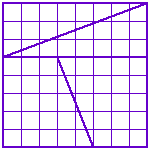
\includegraphics[width=0.22\textwidth]{assets/puzzle_1}
%      }
%      \subcaptionbox{Rectangle.\label{subfig:b_rectangle}}{
%          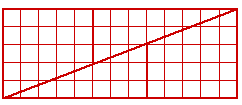
\includegraphics[width=0.35\textwidth]{assets/puzzle_2}
%      }
%      \caption{Example of a figure with subfigures.}
%      \label{fig:puzzles}
% \end{figure}

% References to tables and figures are given as \autoref{fig:tahi} or \autoref{tab:first}. For example, ``We see in \autoref{tab:second} that \ldots'' and ``We see in \autoref{fig:rua} \ldots'' are both correct. Be sure to use the \verb+\label+ command within the figure or table environment and refer to the associated figure or table using \verb+\autoref{your label here}+.

% Please do not use hard-coded figure/table numbers. This is error-prone, and the references will not be hyperlinks.

% Please ensure that your graphics files use standard fonts (Times New Roman, Symbol, etc.) or that those are embedded in the final figure files.
% If they are not embedded, and if the font is not available on the editor's computer, then the font will not be included in the final PDF.
% This may lead to a problem with displaying the final PDF file on computers without an appropriate font.
% At best you select a format that allows embedding the fonts in all non-bitmap figure files.

% Including graphics files in your document can be complicated. In general, you have 2 options. Either (a) you use \texttt{.jpg}, \texttt{.png} or \texttt{.pdf} files (\texttt{.eps} files can be also used, provided that the \texttt{epstopdf} package is added in the preamble) or (b) all of your files must be either \texttt{.ps} or \texttt{.eps}.
% Note that there are tools to convert these formats into one another. The main difference between the formats is how they store the images and how well-suited they are for specific graphics. You can choose between bitmap and vector graphics.

% Bitmap graphics are well suited for photographs (\texttt{.jpg} is very common here) or for screenshots (\texttt{.png} is a lossless encoding in contrast to \texttt{.jpg}, and is thus better suited for all those cases where you have sharp edges in your graphics).

% Vector graphics are the encoding to be chosen for all kinds of drawings (diagrams, charts, \ldots). In contrast to bitmap formats, they can be scaled to any size without any loss of sharpness. This makes it possible to read such graphics even if two pages are printed on one sheet of paper, or if the documents are read electronically.

% So what to choose for your \LaTeX\ document? As a rule of thumb, you should always prefer \texttt{.pdf} or \texttt{.eps}.
% In general, these two formats can contain both, bitmap and vector graphics. But there is no need (and no use) to convert your bitmaps to either of these.

% If you follow Option (a), then you must use the \texttt{PDFLaTeX} command to generate your PDF file, as was done with this file. PDFLaTeX is nowadays the standard - so option (a) should be a natural choice. The final file format is PDF.

% If you follow Option (b), then you must use the outdated \texttt{latex - dvips - ps2pdf} route for generating a PDF file. You may run into a problem if using both the \texttt{hyperref} package and the \texttt{graphicx} package; there seems to be a clash there.
% In that case, you might either not use the \texttt{hyperref} package and continue to use \texttt{graphicx}, or continue to use the \texttt{hyperref} package and use the \texttt{epsfig} package in place of the \texttt{graphicx} package.

% If you persevere with \texttt{hyperref} then be sure to use the appropriate version of the \verb+\usepackage+ command; see the preamble in the source of this file for details. See also \autoref{sec:hyper} below. It is important to note that if you remove the \texttt{hyperref} package, then you have to deal with the correct formatting of hyperlinks on your own.

% Whatever option you choose: if you include figures via \texttt{includegraphics}, then please do so without the file ending (e.g., skip \texttt{.pdf}, \texttt{.eps}, \ldots).

% \subsection{Hyperlinks}
% \label{sec:hyper}

% A \emph{hyperlink} specifies a Web address (URL) or an e-mail address. The use of hyperlinks allows authors to give readers access to external electronic information, such as a dynamic simulation or animation. 
% But please note: hyperlinks (to web pages) might not work forever (web pages might be removed), and thus using hyperlinks intensively may make a paper (or parts thereof) less useful in the future. If enough information is provided in the main body of the paper to enable searching for the cited content in any case and if the inclusion of the web address does not hurt the appearance of the paper, then the web address can be included in the main body of the paper itself.

% \textbf{While the use of hyperlinked text is encouraged in the main body of the paper, it is recommended that corresponding web addresses and other identifying information should be provided in the list of references.} For example, instead of spelling out the web address of the conference website, one would refer to the conference website and the corresponding entry in the reference section will spell out the associated web address and other relevant information such as author(s) and/or organization that published the content. This would allow readers to search for the content using the author(s), organization, etc. in case the actual web address is changed. This also allows for a cleaner appearance of the main body of the paper.

% Each hyperlink should be set in the same font as the text. Hyperlinks are \emph{not} underlined. A live hyperlink (or hotlink) - that is, a hyperlink that will activate your Web browser and take it to an external Web site or that will activate your e-mail software for sending a message to a specific e-mail address - should be colored blue. You can see examples of such hyperlinks in this paper. The use of live hyperlinks is at the discretion of the author(s).

% Non-live hyperlinks that is, the hyperlinks that are included for the reader’s information but do not actually invoke the reader’s Web browser or e-mail software should be colored black (use package \texttt{url} and \verb+\url{http://...}+). To use live hyperlinks in a proceedings paper, use the \texttt{hyperref} package. If you are using \texttt{PDFLaTeX} to generate your PDF file then, as was done for this file, you should use the following as the last \verb+\usepackage+ command that is already in the preamble.

% \begin{verbatim}
% \usepackage[pdftex,colorlinks=true,urlcolor=blue,citecolor=black,
% anchorcolor=black,linkcolor=black]{hyperref}
% \end{verbatim}

% On the other hand, if you are using the traditional \texttt{latex - dvips - ps2pdf} route, then users of MiKTeX or PCTeX for Windows should add the command

% \begin{verbatim}
% \usepackage[dvips,colorlinks=true,urlcolor=blue,citecolor=black,
% anchorcolor=black,linkcolor=black]{hyperref}
% \end{verbatim}

% as the last \verb+\usepackage+ command in the preamble, while users of Y\&Y TeX should add the command

% \begin{verbatim}
% \usepackage[dvipsone,colorlinks=true,urlcolor=blue,citecolor=black,
% anchorcolor=black,linkcolor=black]{hyperref}
% \end{verbatim}

% as the last \verb+\usepackage+ command in the preamble.

% In general, the \verb+\usepackage+ command above that works for MiKTeX running on a Windows system should also work for most implementations of \LaTeX\ running on a UNIX or Apple system.
% Thus the hypertext link \href{http://www.scs.org}{conference website}~\cite{SCS} to the conference website can be established by the command

% \begin{verbatim}
% \href{http://www.scs.org}{conference website}~\cite{SCS}
% \end{verbatim}

% It is recommended to add all hypertext references to the \texttt{.bib} file and refer to them from the text as it is done in the example above.

% If the authors use hyperlinked text in the main body of the paper, they must ensure that each hyperlink includes a citation following the hyperlinked text, a corresponding entry is provided in the list of references, and the associated web address displayed for the hyperlink is complete and correct so that a reader who has only a hard copy of the paper can still access the cited material by typing the relevant part of the displayed text of the hyperlink into the address bar of a Web browser. If the authors opt for including the web address in the main body of the text itself, they must ensure that the hyperlink is complete and correct for the same reason. Again, it is recommended that corresponding web addresses and email addresses should be provided in the references.

% If you use the package \texttt{hyperref} as suggested here, and if you use citation commands to handle references, then your citations will
% become click-able hyperlinks (as in this document). The same happens to all the references to equations, figures, and tables. This can aid the reader in navigating the document.


% %\subsection{Citing a Reference}
% %To cite a reference in the text, use the author-date method. Thus,~\citeN{chi89} could also be cited parenthetically~\cite{chi89}. For a work by four or more authors, use an abbreviated form. For example, a work by Banks, Carson, Nelson~and Nicol would be cited in one of the following ways:~\shortciteN{bcnn:simulation} or~\shortcite{bcnn:simulation}.
% %
% %Parenthetical citations are enclosed in parentheses $(~)$, not square brackets $[~]$. The items in a series of such citations are usually separated by commas. If an item in the series of parenthetical citations contains punctuation because (for example) it refers to a work with three or more coauthors, then all items must be separated by semicolons.
% %
% %The following is a list of \textbf{correct} forms of citations:
% %\begin{itemize}
% %\item Brown and Edwards (1993),
% %\item (Brown and Edwards 1993),
% %\item (Smith 1987, Brown and Edwards 1993), and
% %\item (Smith 1987; Arnold, Brown, and Edwards 1992; Brown et al. 1997).
% %\end{itemize}
% %
% %The following is a list of \textbf{incorrect} forms of citations:
% %\begin{itemize}
% %\item Brown and Edwards [1993],
% %\item (Brown and Edwards, 1993),
% %\item (Smith 1987; Brown and Edwards, 1993), and
% %\item (Smith 1987, Arnold Brown and Edwards 1992, Brown et al. 1995)
% %\end{itemize}
% %
% %For further details, please refer to \emph{The Chicago Manual of Style}~\cite{chicago03}. In \autoref{sec:bibtex} you can see how correct citations can easily be achieved by using \BibTeX.
% %
% %\subsection{List of References}
% %Place the list of references after the appendices. The section heading is \textbf{REFERENCES}, and is not numbered. List only references that are cited in the text. Arrange the references in alphabetical order (chronologically for a particular author or group of authors); do not number the references.
% %Give complete references without abbreviations. To identify multiple references by the same authors and year, append a lower case letter to the year of publication, for example, 1984a and 1984b. Use hanging indentation to distinguish individual entries. Do not insert additional space between references.
% %
% %You can enter the references using (a) \emph{\BibTeX\ as discussed in \autoref{sec:bibtex}}, (b) using the environment \texttt{thebibliography} via the \verb+\bibitem+ and \verb+\cite+ commands, or (c) the \texttt{hangref} environment as shown below.
% %Please note that neither (b) nor (c) are recommended. These alternatives may mean extra work for you and the editor during the editing process. Option (c) means in addition that the references will not be hyperlinks - as the proceedings are electronic proceedings this is not recommended at all.
% %
% %\emph{Whatever you do: the list of entries/items need to be included in your submission! And it needs to be included in such a way that the document can be compiled by the editor.}
% %
% %The bibliographic style for a journal article is: \\
% %\textless{}Surname of first author\textgreater{}, \textless{}First author initials\textgreater{},
% %\textless{}Initials and surnames of other authors\textgreater{}. \textless{}year\textgreater{}.
% %\textless{}Capitalized article title in quotes\textgreater{}. \textless{}\emph{Journal Name in
% %Headline Italics}\textgreater\ \textless{}Volume number\textgreater{}, \textless{}page numbers\textgreater{}.
% %
% %The format for other types of reference can be inferred from the examples in the references, which include:
% %\begin{itemize}
% %\item a technical report~\cite{chi89},
% %\item a proceedings article~\cite{cheng:input94},
% %\item a journal article~\cite{gupta:mnormal},
% %\item a book by 2 authors~\cite{hammersley:montecarlo},
% %\item a chapter in a book~\cite{sch79},
% %\item an unpublished thesis or dissertation~\cite{ste99},
% %\item a book with no identified authors~\cite{chicago03}, and
% %\item a document available on the web~\cite{SCS}.
% %\end{itemize}
% %
% %Be sure that references include all of the necessary information such as full name of the publication, year, name of the proceedings, journal or book title, page numbers, etc.
% %
% %Again, for further details and examples, please refer to \emph{The Chicago Manual of Style}~\cite{chicago03}. Please note that the examples given in the reference section of this document are based on the 16th edition of the Chicago Manual of Style. Clarity and consistency should be your primary concern.


% \section{Using \BibTeX}
% \label{sec:bibtex}

% To cite a reference in the text, the \href{https://www.bibtex.com/s/bibliography-style-ieeetran-ieeetran/}{IEEEtran method}~\cite{IEEEtran} is used. 
% You can cite multiple works within the same brackets~\cite{IEEEtran, chi89, bcnn:simulation}.

% Using \BibTeX\ for referencing is the recommended way. Please, do \textbf{not} typeset references and citations manually. Indeed, the references in this document were generated using \BibTeX, so the source for this document serves as an example of how to use \BibTeX\ to meet the formatting requirements.

% One benefit of using \BibTeX\ is that bibliography formatting and referencing can be greatly simplified: the correct citation and reference list style is automatically created. We assume that you already know how to use \BibTeX.

% Software to manage \BibTeX\ files, for example, JabRef (Java based), can support you in managing and creating valid \texttt{bib} files.
% \emph{Please open your bib file with software like JabRef BEFORE you submit your final version. Experience shows that almost all manually edited bib files contain duplicated bib keys (which means a random selection of references), broken entries which usually lead to missing bibliographic information, invalid keys, and last but not least invalid tokens in bib files. Bib files DO NOT support comments. \BibTeX\ should not report any error for your final submitted document.}

% The \BibTeX\ input file \texttt{scsproc.bst} and the \LaTeX\ macros found in \texttt{scsprocbib.tex} are provided, so no other files (apart from your bibliography) are required. The macros in these files have been tested with \LaTeX. The simplest way to write a paper that uses \BibTeX\ is to take the source file for this document and modify it to generate your article.

% \subsection{Set Up the \BibTeX\ Input Files}

% \BibTeX\ requires a bibliography style file (extension \texttt{.bst}) and a bibliography database file (extension \texttt{.bib}).  This is achieved using

% \begin{verbatim}
% \bibliographystyle{assets/scsproc}
% \bibliography{demobib}
% \end{verbatim}

% just before the AUTHOR BIOGRAPHY section.  The file \texttt{demobib}\ in the \verb+\bibliography+ command should be replaced with the base names of your \BibTeX\ \texttt{.bib} files that you use for your bibliography.  \BibTeX\ is then run as usual to create a bibliography file (\texttt{.bbl}).


% \subsection{Use the Citation Macros}

% Use \verb+\cite+ to cite references in the \LaTeX source document. For example,

% \begin{verbatim}
%     \cite{law:simulationc,cheng:queuehetero}
% \end{verbatim} % no space after the comma!
    
% results in the citation~\cite{law:simulationc,cheng:queuehetero}.

% %There are a number of macros available to cite references in the \LaTeX\ source document.  The \verb+\cite+ macro can be used to give a list of references in parentheses.  For example,

% %\begin{verbatim}
% %\cite{law:simulationc,cheng:queuehetero}
% %\end{verbatim} % no space after the comma!
    
% %results in the citation~\cite{law:simulationc,cheng:queuehetero}. A reference that functions as a noun is created with the \verb+\citeN+ macro. For example,
    
% %\begin{verbatim}
% %\citeN{law:simulationc} say \ldots
% %\end{verbatim}
    
% %results in:~\citeN{law:simulationc} say \ldots\,.
    
% %Citations within parentheses do not need the extra parentheses provided by the above citation commands. To suppress the inclusion of extra parentheses, use the \verb+\citeNP+ macro. To obtain (\citeNP{cheng:queuehetero}, \citeNP{law:simulationc}), for example, use:
    
% %\begin{verbatim}
% %(\citeNP{cheng:queuehetero}, \citeNP{law:simulationc}).
% %\end{verbatim}
    
% %When there are four or more authors, the name of the first author should be given along with the text ``et al.''  This can be achieved with the \verb+\shortcite+ macro. To obtain~\shortcite{bcnn:simulation}, for example, use: 
    
% %\begin{verbatim}
% %\shortcite{bcnn:simulation}
% %\end{verbatim}
    
% %The macros \verb+\shortciteN+ and \verb+\shortciteNP+ are also available to obtain `et al.' when a citation with many authors is used as a noun.
    
% %When citing a reference inside a figure or table caption, please use \verb+\protect\cite+ sequence to avoid build errors.
% %}

% \subsection{Generate the Bibliography File}

% Run \texttt{PDFLaTeX} (or \LaTeX), then \BibTeX, and then \texttt{PDFLaTeX} two more times. Running \texttt{PDFLaTeX} the first time creates the \texttt{.aux} file. Running \BibTeX\ creates the \texttt{.bbl} file.  Running \texttt{PDFLaTeX} again (twice) fixes the bibliography and citation references.


% \subsection{Include the Bibliography File in Your Submission}
% \label{sec:submitbib}

% \textcolor{red}{Be sure to include your \texttt{.bib} file(s) or your \texttt{.bbl} file as part of your submission}. If you only include the \texttt{.bbl} file, then please verify that you include the most up-to-date version reflecting changes during the editing process by rerunning \BibTeX\ one last time before submission.

% Please be aware that submitting the \texttt{.bbl} file instead of the \texttt{.bib} file means extra work for the editing team and for you, as any changes to the reference list need to be done by you in this case.
% Please open and save the file before every submission with software like JabRef to see whether the file is correct and to check for duplicated entries and/or bib keys in the file.


% \section{Author Checklist}
% We strive for a consistent appearance in all papers published in the proceedings. If you used the template and styles within this author’s kit, then almost all of the requirements in this checklist will be automatically satisfied, and there is very little to check.

% Please \textbf{print a hardcopy of your paper}, and go over your printed paper to make sure it adheres to the following requirements. \textit{Thank you!}

% \begin{enumerate}
% 	\item Abstract
%   \begin{enumerate}
% 	  \item \textcolor{red}{150 or fewer words.}
% 	  \item \textcolor{red}{Provide 3-5 keywords (mandatory).} This set of keywords will identify your paper in indices and databases.
% 	\end{enumerate}
% 	\item Paper Length
%   \begin{enumerate}
% 	  \item At least 5, but no more than 12 pages.
% 	  \item Page size is letter size (8.5’’ x 11’’, or 216 mm x 279 mm).
% 	\end{enumerate}
% 	\item All text is in 11-Point Times New Roman except the title, header, and footer (default in this template).
% 	\item Paper title is in 12-Point Times New Roman \textbf{BOLDFACE ALL CAPS} (default in this template).
% 	\item The paper has been \textcolor{red}{spellchecked using U.S. English}. 
% 	\item Spacing and Margins
%   \begin{enumerate}
% 	  \item Single spaced.
% 	  \item Left and right margins are each 1 inch (default in this template).
% 	  \item Top and bottom margins are according to the template.
% 	  \item Title starts 1.25 inches from the top of the page (default in this template).
% 	\end{enumerate}
% 	\item Section Headings
%   \begin{enumerate}
% 	  \item Left justified and set in \textbf{BOLDFACE ALL CAPS} (default in this template).
% 	  \item Numbered, except for the abstract, acknowledgments, references, and author biographies.
% 	  \item Subsection headings are set in \textbf{Boldface Headline Style} (default in this template).
% 	\end{enumerate}
% 	\item No footnotes or page numbers.
% %	\item The copyright notice on the first page contains the name of the symposium or a track where you want to submit your paper, and the running head on subsequent pages is the surnames of all authors.
% 	\item Multiple authors are formatted correctly.
% 	\item Equations are centered and any equation numbers are in parentheses and right-justified (default).
% 	\item Figures and Tables
%   \begin{enumerate}
% 	  \item All text in figures and tables is readable.
% 	  \item Table captions appear above the table.
% 	  \item Figure captions appear below the figure.
% 	\end{enumerate}
% 	\item Citations and References
%   \begin{enumerate}
% 	  \item \textcolor{red}{Citations are by numbers between brackets} (default \BibTeX). 
% 	  \item References are in the hangref style and are listed in the order they are cited in the text (also default \BibTeX\ setting in this template). 
% 	\end{enumerate}
% 	\item Author biographies are one paragraph per author.
% 	\item Hyperlinks
%   \begin{enumerate}
% 	  \item Be sure that hyperlinks will probably work in the future as well.
% 	  \item Live hyperlinks are blue. Nonlive hyperlinks are black (default in this template).
% 	\end{enumerate}
% 	\item All fonts must be embedded in the resulting \texttt{.pdf}. If you use \texttt{pdflatex}, this should already be true--unless you included figures in the \texttt{.eps} or \texttt{.pdf} format which may introduce additional font dependencies. You can use the \texttt{pdffonts} command to see if all the fonts are embedded (the column ``emb'' should say yes for all rows). You can use GhostScript to force embed the fonts, like so: {\texttt{gs -dNOPAUSE -dBATCH -sDEVICE=pdfwrite -dEmbedAllFonts=true -sOutputFile=out.pdf -f in.pdf}} (in Windows, use \texttt{gswin32} or \texttt{gswin32c} to invoke GhostScript).
% \end{enumerate}

% After verifying that your paper meets these requirements, please go to the final submission page at the conference website and submit your paper. Be sure to complete the transfer of copyright form and upload the \texttt{.pdf} receipt. \textit{Thank you for contributing to the SCS conferences!}


% \section*{Acknowledgments}

% Place the acknowledgments section, if needed, after the main text, but before any appendices and references. The section heading is not numbered. These instructions are adapted from the version by Roeder, T. M. K., Frazier, P. I., Wotton, H., Szechtman, R., Yooh, H. L., Harker, J., and Zhou, E. Those instructions were adapted from WSC instructions with permission from WSC BoD~\cite{WSC} that have been iteratively updated and improved by proceedings editors and several other individuals, who are too numerous to name separately since the first set of instructions were written by Barry Nelson for the 1991 WSC.

% \appendix

% \section{Appendices} \label{app:quadratic}
% Place any appendices after the acknowledgments. Note that the default style labels them A, B, C, and so forth (please, do not change this). 
% The solution to \eqref{eq:quadratic} has the form:

% \begin{equation} \label{eq:quadratic sol}
% x = \frac{-b \pm \sqrt{b^2-4ac}}{2a} \mbox{ if } a \ne 0\;.
% \end{equation}


% \section{Getting Help}
% If you need help in preparing your paper, contact the proceedings editors. You can reach the entire team by writing to our unified point of contact at \href{mailto://scs@scs.org}{scs@scs.org}. 


% \section{Most Observed Mistakes}

% The following list comprises \textbf{the most common sources of error} that had to be corrected by previous editors. Please make sure to go through the following list and check that your paper is formatted correctly:
% \begin{enumerate}
% 	\item	The paper is less than 5 or more than 12 pages long.
% 	\item	Paper title and section titles are in \textbf{BOLD ALL CAPS}, subsections are \textbf{Bold and Capitalize the First Letter of Important Words}. Please use the templates.
% 	\item	Paper is in A4 format, not letter format. Please use the required margins.
% 	\item	The copyright notice is incorrect.
% 	\item	The running heads are incorrect. Do not forget that the LastNameLastAuthor is preceded by ``, and ''.
% 	\item	The citation format is incorrect. Use \BibTeX\ for citations and do not change the format used by the template.
% 	\item	The biographies are missing. Do not forget the ``author biographies'' section.
% 	\item	Figures or tables are not referenced in the text or have the incorrect caption format.
% 	% \item	The author section after the title is not formatted correctly, the number of organizations does not define the number of blocks, or the number of blocks does not define the layout.
% 	\item In the heading on the title page, country names are in all capitals.
% 	\item	Paragraphs are not indented.
% 	\item Some fonts in the resulting \texttt{.pdf} are not embedded.
% \end{enumerate}






% Please don't change the bibliographystyle style
\bibliographystyle{scsproc}

% AUTHOR: Include your bib file here
% \bibliography{assets/demobib}
\bibliography{references.bib}


\section*{Author Biographies}

% \textcolor{red}{A biography is mandatory for each author}. A biography starts with an author's name, then provides their position and a brief summary of their research interests. The biography ends with the email. The biography is not intended to be a comprehensive summary of accomplishments. \textcolor{red}{Note that initial submissions are double blind, so biographies must not be included when submitting your manuscript.} Leave space for biographies so that you can include them when submitting the camera-ready version of your paper, after acceptance.

\textbf{\uppercase{Jose Tupayachi}}, UTK graduate student, with expertise in digital transformation, simulation, and machine learning. With a background in information technologies and two years in the industry, Jose has consistently engineered cutting-edge solutions that are both scalable and efficient, effectively tackling complex technical challenges. His areas of interest extend across a diverse spectrum of programming languages and development frameworks, including but not limited to Python, Java, and SQL.

\textbf{\uppercase{Xueping Li}} is a Professor and Dan Doulet Faculty Fellow in the Department of Industrial and Systems Engineering, Co-Director of the Health Innovation Technology and Simulation (HITS) Lab, and the Director of the Ideation Laboratory (iLab) at the University of Tennessee - Knoxville. His research areas include complex system modeling, simulation, and optimization with broad applications in supply chain logistics, healthcare, and energy systems. His research has been sponsored by federal agencies including NSF, NIH, DOE, and HRSA, and other industry partners. He has over 150 peer-reviewed publications and 10 invention disclosures. He is an IISE Fellow and a member of IEEE and INFORMS, and the Past President of the Modeling of Simulation Division of IISE.
% is an Assistant Professor in the Department of Computer Engineering and Software Engineering at Polytechnique Montr\'{e}al, Canada. Previously, he was a post-doctoral researcher at the University of Montr\'{e}al, Canada and at the University of Antwerp, Belgium. He received his PhD at McGill University. His research interests include digital twins, knowledge representation, cyber-physical system verification, model-driven engineering, and model transformations. His email address is \email{bentley.oakes@polymtl.ca}.


\end{document}
